% !TEX root
%
% Copyright (c) 2018  UAVCAN Development Team
%

\documentclass{uavcandoc}

\usepackage{multirow}
\usepackage{tabularx}
\usepackage{amsmath}
\usepackage{amsfonts}
\usepackage{longtable}

% To be removed when ready for publication
\usepackage{draftwatermark}
\SetWatermarkScale{1.2}
\SetWatermarkLightness{0.9}

\urlstyle{same}

% This macro embeds the selected DSDL definition or the contents of a DSDL namespace into the document.
% It accepts one mandatory argument which is either a full DSDL type name, e.g. uavcan.node.Heartbeat,
% or a full type name glob expression, e.g., uavcan.node.*.
\newcommand{\DSDL}[1]{%
    % Clean up beforehand to ensure clean initial state.
    \immediate\write18{rm -f ../*.tmp}%
    % Invoke the target command and save the useful output into a file; ignore error output
    \immediate\write18{../render_dsdl.py #1 > ../dsdl.tmp}%
    % Now, if the above command has failed, the output file would be empty. We remove empty file to escalate error.
    % Escalation is very important as it allows us to abort compilation on failure instead of generating invalid
    % documents silently.
    \immediate\write18{find .. -type f -name '*.tmp' -size 0 -delete}%
    % Read the file. This command fails if the file was empty, which is exactly want we want.
    \immediate\chapter{Data structure description language}\label{sec:dsdl}

\section{General principles}

\section{Language specification}

\subsection{Structure}

Every data type is located in a namespace.
Namespaces may be included into higher-level namespaces, forming a tree hierarchy.

A namespace that is at the root of the tree hierarchy (i.e., not nested within another one)
is called a \emph{root namespace}.
A namespace that is located inside another namespace is called a \emph{nested namespace}.

A data type is uniquely identified by its namespaces and its \emph{short name}.
The short name of a data type is the name of the type itself excluding the containing namespaces.

A \emph{full name} of a data type consists of its short name and all of the outer namespace names.
The short name and the namespace names included in a full name are called \emph{name components}.
Name components are ordered: the root namespace is always the first component of the name,
followed by the nested namespaces, if there are any, in the order of their nesting;
the short name is always the last component of the full name.
The full name is formed by joining its name components via the ASCII dot character ``\verb|.|'' (ASCII code 46).

A \emph{full namespace} is formed by joining together all name components except the short name.

A \emph{sub-root namespace} is the nested namespace that is nested inside the root namespace.
Data types that reside directly under a root namespace do not have a sub-root namespace.

The name structure is illustrated on the figure \ref{fig:dsdl_data_type_name_structure}.

\begin{figure}[H]
    $$
    \overbrace{
        \underbrace{
            \underbrace{\texttt{\huge{uavcan}}}_{\substack{\text{root} \\ \text{namespace}}}%
            \texttt{\huge{.}}%
            \underbrace{\texttt{\huge{node}}}_{\substack{\text{nested, also} \\ \text{sub-root} \\ \text{namespace}}}%
            \texttt{\huge{.}}%
            \underbrace{\texttt{\huge{port}}}_{\substack{\text{nested} \\ \text{namespace}}}%
        }_{\text{full namespace}}%
        \texttt{\huge{.}}%
        \underbrace{\texttt{\huge{GetInfo}}}_{\text{short name}}
    }^{\text{full name}}
    $$
    \caption{Data type name structure.\label{fig:dsdl_data_type_name_structure}}
\end{figure}

Every data type definition is assigned a major and minor version number pair.
In order to uniquely identify a data type definition, its version numbers must be specified.

\subsection{File hierarchy}

\subsection{Syntax}


\section{Data serialization}\label{sec:dsdl_data_serialization}

The main design principle behind the serialized representations described in this section is
the maximization of compatibility with native representations used by currently existing and
likely future computer microarchitectures.
The goal is to ensure that the serialized representations defined by DSDL match internal data representations of
modern computers, so that, ideally, a typical system will not have to perform any data conversion whatsoever while
exchanging data over a UAVCAN network.

\newcommand{\hugett}[1]{\texttt{\huge{#1}}}

\subsection{General principles}

The smallest atomic data entity is a bit.
Eight bits form one byte;
within the byte, the bits are ordered so that the most significant bit is considered first (0-th index),
and the least significant bit is considered last (7-th index).

Numeric values consisting of multiple bytes are encoded so that the least significant byte is encoded first;
such format is also known as little-endian.

\begin{figure}[H]
    $$
    \overset{\text{bit index}}{%
        \underbrace{%
            \overset{0}{\hugett{0}}\quad
            \overset{1}{\hugett{1}}\quad
            \overset{2}{\hugett{0}}\quad
            \overset{3}{\hugett{1}}\quad
            \overset{4}{\hugett{0}}\quad
            \overset{5}{\hugett{1}}\quad
            \overset{6}{\hugett{0}}\quad
            \overset{7}{\hugett{1}}\quad
        }_{\substack{\text{0-th byte} \\ \text{least significant byte}}}%
    }
    \hugett{\ldots}
    \overset{\text{bit index}}{%
        \underbrace{%
            \overset{8n+0}{\hugett{0}}\quad
            \overset{8n+1}{\hugett{1}}\quad
            \overset{8n+2}{\hugett{0}}\quad
            \overset{8n+3}{\hugett{1}}\quad
            \overset{8n+4}{\hugett{0}}\quad
            \overset{8n+5}{\hugett{1}}\quad
            \overset{8n+6}{\hugett{0}}\quad
            \overset{8n+7}{\hugett{1}}\quad
        }_{\substack{n\text{-th byte} \\ \text{most significant byte}}}%
    }
    $$
    \caption{Bit ordering and grouping.\label{fig:dsdl_serialization_bit_ordering}}
\end{figure}

Upon completion, a bit sequence must be appended with zero (0) bits at the end until the total length of
the bit sequence is an integer multiple of eight (8).
The transport layer may introduce additional padding bytes (as opposed to bits) of arbitrary values,
as described in relevant sections of chapter \ref{sec:transport_layer}.
When a serialized representation is deconstructed, the values of the padding bits must be ignored.

\subsection{Void types}

The serialized representation of a void-typed field attribute is constructed as a sequence of zero bits.
The length of the sequence equals the numeric suffix of the type name.

When a void-typed field attribute is decoded, the values of respective bits are ignored;
in other words, any bit sequence of correct length is a valid encoded representation of a void-typed field attribute.
This behavior facilitates usage of void fields as placeholders for non-void fields
introduced in newer versions of the data type (section \ref{sec:dsdl_versioning}).

\begin{remark}
    The following data schema will be encoded as a sequence of three zero bits $000_2$
    (five trailing padding bits not included):
    \begin{minted}{python}
        void3
    \end{minted}
    The following bit sequences are valid encoded representations of the schema:
    $000_2$,
    $001_2$,
    $010_2$,
    $011_2$,
    $100_2$,
    $101_2$,
    $110_2$,
    $111_2$.
\end{remark}

\subsection{Primitive types}

\subsubsection{Boolean types}

The serialized representation of a value of type \verb|bool| is a single bit.
If the value represents falsity, the value of the bit is zero (0); otherwise, the value of the bit is one (1).

\subsubsection{Unsigned integer types}\label{sec:dsdl_serialized_unsigned_integer}

The serialized representation of an unsigned integer value of length $n$ bits
(which is reflected in the numerical suffix of the data type name)
is constructed as if the number were to be written in base-2 numerical system
with leading zeros preserved so that the total number of binary digits would equal $n$.

\begin{remark}
    The serialized representation of integer 123 of type \verb|uint9| is $001111011_2$.
\end{remark}

\subsubsection{Signed integer types}

The serialized representation of a non-negative value of a signed integer type is constructed as described
in section \ref{sec:dsdl_serialized_unsigned_integer}.

The serialized representation of a negative value of a signed integer type is computed by
applying the following transformation:
$$2^n + x$$
where $n$ is the bit length of the serialized representation
(which is reflected in the numerical suffix of the data type name)
and $x$ is the value whose serialized representation is being constructed.
The result of the transformation is a positive number,
whose serialized representation is then constructed as described in section \ref{sec:dsdl_serialized_unsigned_integer}.

The representation described here is widely known as \emph{two's complement}.

\begin{remark}
    The serialized representation of integer -123 of type \verb|int9| is $110000101_2$.
\end{remark}

\subsubsection{Floating point types}

The serialized representation of floating point types follows the IEEE 754 series of standards as follows:

\begin{itemize}
    \item \verb|float16| --- IEEE 754 binary16;
    \item \verb|float32| --- IEEE 754 binary32;
    \item \verb|float64| --- IEEE 754 binary64.
\end{itemize}

\subsection{Nested data structures}

Nested data structures are serialized directly in-place,
as if their DSDL definition was pasted directly in place of their reference.
No additional prefixes, suffixes, or padding is provided.

\subsection{Fixed size arrays}

Fixed-size arrays are serialized as a plain sequence of items,
with each item serialized independently in place, with no alignment.
No extra data is added.

Essentially, a fixed-size array of size $X$ elements will be serialized exactly in the same way
as a sequence of $X$ fields of the same type in a row.
Hence, the following two data type definitions will have identical binary representation,
the only actual difference being their representation for the application
if automatic code generation is used.

\begin{minted}{python}
AnyType[3] array
\end{minted}

\begin{minted}{python}
AnyType item_0
AnyType item_1
AnyType item_2
\end{minted}

\subsection{Dynamic arrays}

The following two array definitions are equivalent;
the difference is their representation in the DSDL definition for better readability:
\begin{minted}{python}
AnyType[<42] a      # Can contain from 0 to 41 elements
AnyType[<=41] b     # Can contain from 0 to 41 elements
\end{minted}

A dynamic array is serialized as a sequence of serialized items prepended with an unsigned
integer field representing the number of contained items - the \emph{length field}.
The bit width of the length field is a function of the maximum number of items in the array:
$$\lceil{}\log_2 (X + 1)\rceil{}$$
where $X$ is the maximum number of items in the array.
For example, if the maximum number of items is 251, the length field bit width must be 8 bits;
if the maximum number of items is 1, the length field bit width will be just a single bit.

It is recommended to manually align dynamic arrays by prepending them with void fields
so that the first element is byte-aligned, as that enables more efficient serialization and
deserialization.
This recommendation does not need to be followed if the size of the array elements is not
a multiple of eight bits or if the array elements are of variable size themselves
(e.g., a dynamic array of nested types which contain dynamic arrays themselves).

Consider the following definition:

\begin{minted}{python}
void2                       # Padding - not required, provided as an example
AnyType[<42] array          # The length field is 6 bits wide (see the formula)
\end{minted}

If the array contained three elements,
the resulting binary representation would be equivalent to that of the following definition:

\begin{minted}{python}
void2                       # Padding - not required, provided as an example
uint6 array_length          # Set to 3, because the array contains three elements
AnyType item_0
AnyType item_1
AnyType item_2
\end{minted}

\subsection{Unions}

Similar to dynamic arrays, tagged unions are serialized as two subsequent entities:
the union tag followed by the selected field, with no additional data.

The union tag is an unsigned integer, the bit length of which is a function of the number of fields in the union:
$$\lceil{}\log_2 N\rceil{}$$
where N is the number of fields in the union.
The value serialized in the union tag is the index of the selected field.
Field indexes are assigned according to the order in which they are defined in DSDL,
starting from zero;
i.e. the first defined field has the index 0, the second defined field has the index 1, and so on.

Constants are not affected by the union tag.

It is recommended to manually align unions when they are nested into outer data types by
prepending them with void fields so that the elements are byte-aligned,
as that enables more efficient serialization and deserialization.

Consider the following example:

\begin{minted}{python}
@union                  # In this case, the union tag requires 2 bits
uint16  FOO = 42        # A regular constant attribute
uint16  a               # Index 0
uint8   b               # Index 1
float64 c               # Index 2
uint32  BAR = 42        # Another regular constant
\end{minted}

In order to encode the field \verb|b|, which, according to the definition,
has the data type \verb|uint8|, the union tag should be assigned the value 1.
The following structure will have an identical layout:

\begin{minted}{python}
uint2 tag               # Set to 1
uint8 b                 # The actual data
\end{minted}

If the value of \verb|b| was 7, the resulting serialized byte sequence would be (in binary):
$$%
\underbrace{\texttt{01}}_{\text{tag}}%
\overbrace{\texttt{000001 11}}^{\text{field }\texttt{b}}%
\underbrace{\texttt{000000}}_{\text{padding}}%
$$

\subsection{Composite types}

A serialized representation of an object of composite type $T$ is an ordered set of serialized representations of
its field attribute values joined into a bit string.
The ordering of the serialized representations of the field attribute values follows the order
of field attribute declaration of $T$.

Bit strings do not have any implicit entities such as padding or headers.
Data type developers are advised\footnote{But not required.} to manually align field attributes at
byte boundaries using padding field attributes in order to simplify data layouts
and improve the performance of serialization and deserialization routines.

\begin{remark}
    Consider the following data schema definition,
    where the fields are assigned runtime values shown in the comments:

    \begin{minted}{python}
        #                          decimal    bit string            comment
        truncated uint12 first   # +48858     1011_1110_1101_1010   overflow, MSB truncated
        truncated int3   second  # -1         111                   two's complement
        truncated int4   third   # -5         1011                  two's complement
        truncated int2   fourth  # -1         11                    two's complement
        truncated uint4  fifth   # +136       1000_1000             overflow, MSB truncated
    \end{minted}

    It can be seen that the bit layout is rather complicated because the field boundaries do not align with byte
    boundaries, which makes it a good case study.
    The resulting serialized byte sequence is shown below in the base-2 system,
    where bytes (octets) are comma-separated:

    $$
        \overbrace{\hugett{11011010,1110}}^{\texttt{first}}%
        \underbrace{\hugett{111}}_{\texttt{second}}%
        \overbrace{\hugett{1,011}}^{\texttt{third}}%
        \underbrace{\hugett{11}}_{\texttt{fourth}}%
        \overbrace{\hugett{100,0}}^{\texttt{fifth}}%
        \underbrace{\hugett{0000000}}_{\substack{\text{Implicit padding} \\ \text{to 8-bit alignment}}}
    $$
\end{remark}

\section{Data type compatibility and versioning}\label{sec:dsdl_versioning}

\subsection{Rationale}

Data type definitions may evolve over time as they are refined to better address the needs of their applications.
UAVCAN defines a set of rules that allow data type designers to modify and advance their
data type definitions while ensuring backward compatibility and functional safety.

\subsection{Compatibility}

\subsubsection{Bit compatibility}

A data type or schema $A$ is bit-compatible with a data type or schema $B$ if and only if
the set of serialized representations\footnote{The serialization rules are reviewed
in detail in the section \ref{sec:dsdl_data_serialization}.}
of $A$ is a superset of the set of serialized representations of $B$.

$A$ and $B$ are said to be \emph{mutually bit-compatible} if
their sets of serialized representations are equal.

A \emph{variable-length} data type or schema is a serializable data type or schema
whose set of serialized representations contains bit sequences of different lengths.
Conversely, any data type or schema that is not variable-length is \emph{fixed-length}.

\begin{remark}[breakable]
    The following two definitions are mutually bit-compatible:

    \begin{minted}{python}
        uint32 a
        uint32 b
    \end{minted}

    \begin{minted}{python}
        uint64 c
    \end{minted}

    Consider the following example data type definition; assume that its full data type name is
    \verb|demo.Pair|:

    \begin{minted}{python}
        # demo.Pair.1.0
        float16 first
        float16 second
    \end{minted}

    Further, let the following define a data type named \verb|demo.PairVector|:

    \begin{minted}{python}
        # demo.PairVector.1.0
        demo.Pair.1.0[3] vector
    \end{minted}

    Then the following two definitions are bit-compatible:

    \begin{minted}{python}
        demo.PairVector.1.0 pair_vector
    \end{minted}

    \begin{minted}{python}
        float16 first_0     # pair_vector.vector[0].first
        float16 second_0    # pair_vector.vector[0].second
        float16 first_1     # pair_vector.vector[1].first
        float16 second_1    # pair_vector.vector[1].second
        float16 first_2     # pair_vector.vector[2].first
        float16 second_2    # pair_vector.vector[2].second
    \end{minted}

    The latter definition in the example above is a flattened unrolled form of the former definition.
    As such, in that particular example, both definitions can be used interchangeably;
    an object serialized using one definition can be deserialized using the other definition.
    However, it is also possible to construct bit-compatible definitions that are not functionally equivalent:

    \begin{minted}{python}
        float16 a
        float32 b
    \end{minted}

    \begin{minted}{python}
        float32 a
        float16 b
    \end{minted}

    Even though the above definitions are bit-compatible, one cannot be substituted with the other.
    The problem of functional equivalency is addressed by the concept of semantic compatibility,
    explored in the section \ref{sec:dsdl_semantic_compatibility}.

    Complicated scenarios are possible when a bit belonging to a primitive-typed field attribute
    is handed over to a constrained field such as an implicit array length field or an implicit union tag field.
    Some interesting examples are shown in the table \ref{table:dsdl_many_compat},
    together with a set of serialized representation patterns.
    Remember that the bits belonging to void-typed field attributes are ignored during deserialization.

    % Please do not remove the hard placement specifier [H], it is needed to keep tables ordered.
    \begin{table}[H]\caption{Complex bit compatibility examples}\label{table:dsdl_many_compat}
        \begin{tabu}{|l|X|X|X|X|X|}
            \hline
            \rowfont{\bfseries}
            &A                  &  B                &  C                &  D                &  E                 \\
            \hline

            \multirow{2}{*}{\textbf{Definition}}
            &\texttt{void1}     &\texttt{bool x}    &\texttt{void1}     &\texttt{bool x}    &\texttt{bool[<5] a} \\
            &\texttt{bool[<3] a}&\texttt{bool[<3] a}&\texttt{bool[<4] a}&\texttt{bool[<4] a}&                    \\
            \hline

            \multirow{8}{*}{%
                \begin{tabular}[x]{@{}l@{}}\textbf{Serialized}\\\textbf{representations}\end{tabular}%
            }
            &\multicolumn{2}{l|}{\texttt{000   }}   &\multicolumn{2}{l|}{\texttt{000    }}  &\texttt{000     } \\
            &\multicolumn{2}{l|}{\texttt{001a  }}   &\multicolumn{2}{l|}{\texttt{001a   }}  &\texttt{001a    } \\
            &\multicolumn{2}{l|}{\texttt{010aa }}   &\multicolumn{2}{l|}{\texttt{010aa  }}  &\texttt{010aa   } \\
            &\multicolumn{2}{l|}{\texttt{      }}   &\multicolumn{2}{l|}{\texttt{011aaa }}  &\texttt{011aaa  } \\
            &\multicolumn{2}{l|}{\texttt{100   }}   &\multicolumn{2}{l|}{\texttt{100    }}  &\texttt{100aaaa } \\
            &\multicolumn{2}{l|}{\texttt{101a  }}   &\multicolumn{2}{l|}{\texttt{101a   }}  &\texttt{        } \\
            &\multicolumn{2}{l|}{\texttt{110aa }}   &\multicolumn{2}{l|}{\texttt{110aa  }}  &\texttt{        } \\
            &\multicolumn{2}{l|}{\texttt{      }}   &\multicolumn{2}{l|}{\texttt{111aaa }}  &\texttt{        } \\
            \hline

            {\begin{tabular}[x]{@{}l@{}}\textbf{Bit-compatible}\\\textbf{with}\end{tabular}}
            &B                  & A                 & A, B, D           & A, B, C           & \emph{(none)}    \\
            \hline
        \end{tabu}
    \end{table}
\end{remark}

\subsubsection{Semantic compatibility}\label{sec:dsdl_semantic_compatibility}

A data type $A$ is semantically compatible with a data type $B$
if an application that correctly uses $A$ exhibits a functionally equivalent behavior to an application
that correctly uses $B$.
The property of semantic compatibility is commutative.

\begin{remark}[breakable]
    Despite using different binary layouts, the following two definitions are semantically compatible
    and also bit-compatible:

    \begin{minted}{python}
        uint16 FLAG_A = 1
        uint16 FLAG_B = 256
        uint16 flags
    \end{minted}

    \begin{minted}{python}
        uint8 FLAG_A = 1
        uint8 FLAG_B = 1
        uint8 flags_a
        uint8 flags_b
    \end{minted}

    Therefore, the definitions can be used interchangeably.
    It should be noted here that due to different set of field and constant attributes,
    the source code auto-generated from the provided definitions may be not drop-in replaceable,
    requiring changes in the application;
    however, source-code-level application compatibility is orthogonal to data type compatibility.
\end{remark}

\subsection{Versioning}

\subsubsection{General assumptions}

The concept of versioning applies only to composite data types.
As such, unless specifically stated otherwise, every reference to ``data type''
in this section implies a composite data type.

A data type is uniquely identified by its full name,
assuming that every root namespace is uniquely named.
There is one or more versions of every data type.

A data type definition is uniquely identified by its full name and the version number pair.
In other words, there may be multiple definitions of a data type differentiated by their version numbers.

\subsubsection{Versioning principles}

Every data type definition has a pair of version numbers ---
a major version number and a minor version number, following the principles of semantic versioning.

For the purposes of the following definitions, a \emph{release} of a data type definition stands for
the disclosure of the data type definition to its intended users or to the general public,
or for the commencement of usage of the data type definition in a production system.

In order to ensure a deterministic application behavior and ensure a robust migration path
as data type definitions evolve, UAVCAN requires that all data type definitions that share the same
full name and the same major version number must be semantically compatible with each other
and mutually bit-compatible with each other.

The versioning rules do not extend to scenarios where the name of a data type is changed,
because that would essentially construe the release of a new data type,
which relieves its designer from all compatibility requirements.
When a new data type is first released,
the version numbers of its first definition must be assigned ``1.0'' (major 1, minor 0).

In order to ensure predictability and functional safety of applications that leverage UAVCAN,
the standard requires that once a data type definition is released,
its DSDL source text, name, version numbers, fixed port-ID, and other properties cannot undergo any
modifications whatsoever, with the following exceptions:
\begin{itemize}
    \item Whitespace changes of the DSDL source text are allowed,
    excepting string literals and other semantically sensitive contexts.

    \item Comment changes of the DSDL source text are allowed as long as such changes
    do not affect semantic compatibility of the definition.

    \item A deprecation marker directive (section~\ref{sec:dsdl_directives}) can be added or removed\footnote{%
    Removal is useful when a decision to deprecate a data type definition is withdrawn.}.
\end{itemize}
Addition or removal of the fixed port identifier is not permitted after a data type definition
of a particular version is released.

Therefore, substantial modifications of released data types are only possible by releasing
new definitions of the same data type.
If it is desired and possible to keep the same major version number for a new definition of the data type,
the minor version number of the new definition shall be one greater than the newest existing minor version
number before the new definition is introduced.
Otherwise, the major version number shall be incremented by one and the minor version shall be set to zero.

An exception to the above rules applies when the major version number is zero.
Data type definitions bearing the major version number of zero are not subjected to any compatibility requirements.
Released data type definitions with the major version number of zero are permitted to change in arbitrary
ways without any regard for compatibility.
It is recommended, however, to follow the principles of immutability, releasing every subsequent definition
with the minor version number one greater than the newest existing definition.

For any data type, there shall be at most one definition per version.
In other words, there must be exactly one or zero definitions
per combination of data type name and version number pair.

All data types under the same name must be also of the same kind.
In other words, if the first released definition of a data type is of the message kind,
all other versions must also be of the message kind.

\subsubsection{Fixed port identifier assignment constraints}

The following constraints apply to fixed port-ID assignments:
\begin{align*}
    \exists P(x_{a.b})                          &\rightarrow \exists P(x_{a.c})
    &\mid&\ b < c;\ x \in (M \cup S)
    \\
    \exists P(x_{a.b})                          &\rightarrow         P(x_{a.b}) =    P(x_{a.c})
    &\mid&\ b < c;\ x \in (M \cup S)
    \\
    \exists P(x_{a.b}) \land \exists P(x_{c.d}) &\rightarrow         P(x_{a.b}) \neq P(x_{c.d})
    &\mid&\ a \neq c;\ x \in (M \cup S)
    \\
    \exists P(x_{a.b}) \land \exists P(y_{c.d}) &\rightarrow         P(x_{a.b}) \neq P(y_{c.d})
    &\mid&\ x \neq y;\ x \in T;\ y \in T;\ T = \left\{ M, S \right\}
\end{align*}
where $t_{a.b}$ denotes a data type $t$ version $a.b$ ($a$ major, $b$ minor);
$P(t)$ denotes the fixed port-ID (whose existence is optional) of data type $t$;
$M$ is the set of message types, and $S$ is the set of service types.

\subsubsection{Non-fixed port identifier assignment recommendations}

For non-fixed port identifiers
it is recommended to ensure that any port identifier of a given kind (subject or service)
is only used with one major version of one data type.

Sharing a port identifier of a given kind with different major versions of the same data type or different data types
is not recommended even if such different types are bit-compatible and semantically compatible
because it may complicate network maintenance and analysis; additionally, it may confuse automated
network analysis software.

The kind is specified above explicitly due to the fact that the sets of subject-ID and service-ID are orthogonal.
In other words,
the numeric value of a port-ID may refer to different data types if they are of different kinds.

\subsubsection{Data type version selection}

DSDL compilers should compile every available data type version separately,
allowing the application to choose from all available major and minor version combinations.

When emitting a transfer, the major version of the data type is chosen at the discretion of the application.
The minor version should be the newest available one under the chosen major version.

When receiving a transfer, the node deduces which major version of the data type to use
from its port identifier (either fixed or non-fixed).
The minor version should be the newest available one under the deduced major version\footnote{%
Such liberal minor version selection policy poses no compatibility risks since all definitions under the same
major version are compatible with each other.}.

It follows from the above two rules that when a node is responding to a service request,
the major data type version used for the response transfer shall be the same that is used for the request transfer.
The minor versions may differ, which is acceptable due to the major version compatibility requirements.

\begin{remark}[breakable]
    A simple usage example is provided in this intermission.

    Suppose a vendor named ``Sirius Cybernetics Corporation'' is contracted to design a
    cryopod management data bus for a colonial spaceship ``Golgafrincham B-Ark''.
    Having consulted with applicable specifications and standards, an engineer came up with the following
    definition of a cryopod status message type (named \verb|sirius_cyber_corp.b_ark.cryopod.Status|):

    \begin{minted}{python}
        # sirius_cyber_corp.b_ark.cryopod.Status.0.1

        float16 internal_temperature    # [kelvin]
        float16 coolant_temperature     # [kelvin]

        # Status flags in the lower bits
        uint8 FLAG_COOLING_SYSTEM_A_ACTIVE = 1
        uint8 FLAG_COOLING_SYSTEM_B_ACTIVE = 2
        # Error flags in the higher bits
        uint8 FLAG_PSU_MALFUNCTION = 32
        uint8 FLAG_OVERHEATING     = 64
        uint8 FLAG_CRYOBOX_BREACH  = 128
        # Storage for the above defined flags (this is not the recommended practice)
        uint8 flags
    \end{minted}

    The definition is then deployed to the first prototype for initial laboratory testing.
    Since the definition is experimental, the major version number is set to zero in order to signify the
    tentative nature of the definition.
    Suppose that upon completion of the first trials it is identified that the units must track their power consumption
    in real time for each of the three redundant power supplies independently.

    It is easy to see that the amended definition shown below is neither semantically compatible nor bit-compatible
    with the original definition; however, it shares the same major version number of zero, because the backward
    compatibility rules do not apply to zero-versioned data types to allow for low-overhead experimentation
    before the system is deployed and fielded.

    \begin{minted}{python}
        # sirius_cyber_corp.b_ark.cryopod.Status.0.2

        truncated float16 internal_temperature    # [kelvin]
        truncated float16 coolant_temperature     # [kelvin]

        saturated float32 power_consumption_0     # [watt] Power consumption by the redundant PSU 0
        saturated float32 power_consumption_1     # [watt] likewise for PSU 1
        saturated float32 power_consumption_2     # [watt] likewise for PSU 2

        # Status flags in the lower bits
        uint8 FLAG_COOLING_SYSTEM_B_ACTIVE = 1
        uint8 FLAG_COOLING_SYSTEM_A_ACTIVE = 2
        # Error flags in the higher bits
        uint8 FLAG_PSU_MALFUNCTION = 32
        uint8 FLAG_OVERHEATING     = 64
        uint8 FLAG_CRYOBOX_BREACH  = 128
        # Storage for the above defined flags (this is not the recommended practice)
        uint8 flags
    \end{minted}

    The last definition is deemed sufficient and is deployed to the production system
    under the version number of 1.0: \verb|sirius_cyber_corp.b_ark.cryopod.Status.1.0|.

    Having collected empirical data from the fielded systems, the Sirius Cybernetics Corporation has
    identified a shortcoming in the v1.0 definition, which is corrected in an updated definition.
    Since the updated definition, which is shown below, is mutually semantically
    compatible\footnote{The topic of data serialization is explored in detail in the section
    \ref{sec:dsdl_data_serialization}.}
    with v1.0, the major version number is kept the same and the minor version number is incremented by one:

    \begin{minted}{python}
        # sirius_cyber_corp.b_ark.cryopod.Status.1.1

        saturated float16 internal_temperature    # [kelvin]
        saturated float16 coolant_temperature     # [kelvin]

        float32[3] power_consumption    # [watt] Power consumption by the PSU

        # Error flags (this is the recommended practice)
        bool flag_cryobox_breach
        bool flag_overheating
        bool flag_psu_malfunction

        void3   # Reserved for other flags

        # Status flags (this is the recommended practice)
        bool flag_cooling_system_a_active
        bool flag_cooling_system_b_active
    \end{minted}

    Since the definitions v1.0 and v1.1 are mutually bit-compatible and semantically compatible,
    UAVCAN nodes using either of them can successfully interoperate on the same bus.

    Suppose further that at some point a newer version of the cryopod module,
    equipped with better temperature sensors, is released.
    The definition is updated accordingly to use \verb|float32| for the temperature fields instead of \verb|float16|.
    Seeing as that change breaks the bit compatibility,
    the major version number has to be incremented by one,
    and the minor version number has to be reset back to zero:

    \begin{minted}{python}
        # sirius_cyber_corp.b_ark.cryopod.Status.2.0

        float32 internal_temperature    # [kelvin]
        float32 coolant_temperature     # [kelvin]

        float32[3] power_consumption    # [watt] Power consumption by the PSU

        # Error flags (this is the recommended practice)
        bool flag_cryobox_breach
        bool flag_overheating
        bool flag_psu_malfunction

        void3   # Reserved for other flags

        # Status flags (this is the recommended practice)
        bool flag_cooling_system_a_active
        bool flag_cooling_system_b_active
    \end{minted}

    Nodes using v1.0, v1.1, and v2.0 definitions can still coexist on the same network,
    and they can interoperate successfully as long as they all support at least v1.x or v2.x.

    In general, nodes that need to maximize their compatibility are likely to employ all existing major versions of
    each used data type.
    If there are more than one minor versions available, the highest minor version within the major version should
    be used in order to take advantage of the latest changes in the data type definition.
    It is also expected that in certain scenarios some nodes may resort to publishing the same message type
    using different major versions concurrently to circumvent compatibility issues
    (in the example reviewed here that would be v1.1 and v2.0).
\end{remark}

\section{Conventions and recommendations}

% Data type comments
% Field comments https://forum.uavcan.org/t/dsdl-documentation-comments/407

%
    % Clean up afterwards to prevent accidental reuse if the command fails the next time we invoke it.
    \immediate\write18{rm -f ../*.tmp}%
}

\title{Specification v1.0}

\hbadness=10000

\begin{document}
\frontmatter

\begin{titlepage}

\section*{Overview}

UAVCAN is an open lightweight protocol designed for reliable communication in aerospace and robotic applications via
robust vehicle bus networks.

Features:

\begin{itemize}
    \item Democratic network - no bus master, no single point of failure.
    \item Publish/subscribe and request/response (RPC\footnote{Remote procedure call}) exchange semantics.
    \item Efficient exchange of large data structures with automatic decomposition and reassembly.
    \item Lightweight, deterministic, easy to implement, and easy to validate.
    \item Suitable for deeply embedded, resource constrained, hard real-time systems.
    \item Supports dual and triply modular redundant transports.
    \item Supports high-precision network-wide time synchronization.
    \item The specification and high quality reference implementations in popular programming languages are free,
    open source, and available for commercial use (MIT license).
\end{itemize}

\BeginRightColumn

\section*{Support and feedback}

Information, documentation, and discussions related to UAVCAN are available via the official website at
\href{http://uavcan.org}{uavcan.org}.

\section*{License}

UAVCAN is a standard open to everyone, and it will always remain this way.
No licensing or approval of any kind is necessary for its implementation, distribution, or use.

% The following statement looks a bit archaic, but it is the recommended form according to
% https://creativecommons.org/choose/results-one?license_code=by&amp;jurisdiction=&amp;version=4.0&amp;lang=en
This work is licensed under the Creative Commons Attribution 4.0 International License.
To view a copy of this license, visit \url{http://creativecommons.org/licenses/by/4.0/}
or send a letter to Creative Commons, PO Box 1866, Mountain View, CA 94042, USA.

\begin{center}
    \includegraphics[width=0.3\textwidth]{cc-by}
\end{center}

\BeginRightColumn

\section*{Disclaimer of warranty}

NOTE WELL: This Specification is provided on an ``AS IS'' BASIS, WITHOUT WARRANTIES OR CONDITIONS OF ANY KIND,
express or implied, including, without limitation, any warranties or conditions of
TITLE, NON-INFRINGEMENT, MERCHANTABILITY, or FITNESS FOR A PARTICULAR PURPOSE.

\BeginRightColumn

\section*{Limitation of liability}

In no event and under no legal theory, whether in tort (including negligence), contract, or otherwise,
unless required by applicable law (such as deliberate and grossly negligent acts) or agreed to in writing,
shall any author of this Specification be liable for damages,
including any direct, indirect, special, incidental, or consequential damages of any character arising
from, out of, or in connection with the Specification or the implementation, deployment,
or other use of the Specification (including but not limited to damages for loss of goodwill,
work stoppage, equipment failure or malfunction, injuries to persons,
or any and all other commercial damages or losses),
even if such author has been advised of the possibility of such damages.

\end{titlepage}

\tableofcontents
\clearpage\onecolumn\listoftables
\clearpage\onecolumn\listoffigures

\mainmatter

\chapter{Introduction}\label{sec:introduction}

This chapter covers the basic concepts that govern development and maintenance of the specification.
The actual specification is contained in the following chapters.

The reader should have a solid understanding of the main concepts and operating principles of the CAN bus.

\section{Core design goals}

UAVCAN is designed to adhere to the following set of basic principles.

\begin{description}
    \item[Democratic network] - There should be no master node.
    All nodes in the network should have the same communication rights; there should be no single point of failure.

    \item[Nodes can exchange long payloads] - Nodes must be provided with a simple way to exchange large
    data structures that cannot fit into a single CAN\footnote{Here and in the following parts of the
    specification, "CAN" implies both CAN 2.0 and CAN FD, unless specifically noted otherwise.}
    frame (such as GNSS solutions, 3D vectors, etc.).
    UAVCAN should perform automatic transfer decomposition and reassembly at the protocol level,
    hiding the related complexity from the application.

    \item[Support for redundant interfaces and redundant nodes] - This is a common requirement for
    safety-critical applications.

    \item[High throughput, low latency communication] - Applications that are dependent on high-frequency,
    hard real-time control loops, require a low-latency, high-throughput communication method.

    \item[Simple logic, low computational requirements] - UAVCAN targets a wide variety of embedded systems,
    from high-performance embedded on-board computers for intensive data processing
    (e.g., a high-performance GNU/Linux-powered machine) to extremely resource-constrained microcontrollers.
    The latter imposes severe restrictions on the amount of logic needed to implement the protocol.

    \item[Common high-level functions should be clearly defined] - UAVCAN defines standard services
    and messages for common high-level functions, such as network discovery, node configuration,
    node software update, node status monitoring (which naturally grows into a vehicle-wide health monitoring),
    network-wide time synchronization, dynamic node ID allocation (a.k.a. plug-and-play node support), etc.

    \item[Open specification and reference implementations] - The UAVCAN specification is open and
    freely available; the reference implementations are distributed under the terms of the permissive MIT License.
\end{description}

\section{Capabilities}

This section summarizes the capabilities of the UAVCAN protocol.

UAVCAN-based networks can accommodate up to 127 nodes on the same logical bus.
More nodes can be added to the system by separating the bus into several independent logical segments
interconnected via gateway nodes.

UAVCAN supports up to 32768 distinct message data types and up to 256 distinct service data types.
Part of those are reserved for the standard data types defined by the specification;
the rest are available for vendor- and application-specific data types.
More information is provided in the chapter \ref{sec:application_layer}.

UAVCAN supports eight distinct communication priority levels,
defined in the section \ref{sec:transfer_prioritization}.
Within each priority level, different types of transfers and different data types are
prioritized in a well-defined deterministic manner.

UAVCAN supports both CAN 2.0 and CAN FD transports.
CAN FD should be considered the primary transport, whereas CAN 2.0 is supported as legacy.
Non-redundant, doubly-redundant and triply-redundant transports are supported.
More information on the transport properties and standardized physical connectivity options
is provided in the chapter \ref{sec:hardware_design_recommendations}.

\section{Specification update and approval process}

The UAVCAN development team is charged with advancing the specification based on the input from adopters.
This feedback is gathered via the official discussion
forum\footnote{Please refer to \href{http://uavcan.org}{uavcan.org}.},
which is open to everyone.

The set of standard data type definitions is one of the cornerstone concepts of the specification
(the data structure description language (DSDL) and related concepts are described in section \ref{sec:dsdl}).
Within the same major version, the specification can be extended only in the following ways:

\begin{itemize}
    \item A new data type can be added, possibly with a default data type ID,
    as long as the default data type ID doesn't conflict with one of the existing data types.

    \item An existing data type can be modified, as long as its version number is updated accordingly
    and the backward compatibility guarantees are respected.

    \item A major version of an existing data type can be declared deprecated.
    \begin{itemize}
        \item Once declared deprecated, the major version will be maintained for at least two more years.
        \item Deprecation will be indicated in the DSDL definition and announced via the discussion forum.
    \end{itemize}

    \item An existing data type can be declared deprecated.
    \begin{itemize}
        \item Once declared deprecated, the data type will be maintained for at least two more years.
        After this period its default data type ID may be reused for an incompatible data type.
        \item Deprecation will be indicated in the DSDL definition and announced via the discussion forum.
    \end{itemize}
\end{itemize}

A link to the repository containing the set of default DSDL definitions can be found on the official
website\footnote{\href{http://uavcan.org}{uavcan.org}}.

\section{Referenced sources}

The UAVCAN specification contains references to the following sources:

\begin{itemize}
    \item CiA 801 - Application note - Automatic bit rate detection.
    \item CiA 103 - Intrinsically safe capable physical layer.
    \item CiA 303 - Recommendation - Part 1: Cabling and connector pin assignment.
    \item IEEE 754 - Standard for binary floating-point arithmetic.
    \item ISO 11898-1 - Controller area network (CAN) - Part 1: Data link layer and physical signaling.
    \item ISO 11898-2 - Controller area network (CAN) - Part 2: High-speed medium access unit.
    \item ISO/IEC 10646 - Universal Coded Character Set (UCS).
    \item ISO/IEC 14882 - Programming Language C++.
    \item "Implementing a Distributed High-Resolution Real-Time Clock using the CAN-Bus", M. Gergeleit and H. Streich.
    \item "In Search of an Understandable Consensus Algorithm (Extended Version)", Diego Ongaro and John Ousterhout.
    \item \href{http://semver.org}{semver.org} - Semantic versioning specification.
\end{itemize}

\chapter{Basic concepts}\label{sec:basic_concepts}


A UAVCAN network is a decentralized peer network, where each peer (node) has a unique
numeric identifier --- \emph{node ID} --- ranging from 1 to 127, inclusively.
Nodes of a UAVCAN network can communicate using the following communication methods:

\begin{description}
    \item[Message broadcasting] --- The primary method of data exchange with one-to-all publish/subscribe semantics.
    \item[Service invocation] --- The communication method for peer-to-peer request/response
    interactions\footnote{Like remote procedure call (RPC).}.
\end{description}

For each type of communication, a predefined set of data structures is used,
where each data structure has a unique identifier --- the \emph{data type ID} (DTID).
Additionally, every data structure definition has a pair of major and minor semantic version numbers,
which enable data type definitions to evolve in arbitrary ways while ensuring a well-defined
migration path if backward-incompatible changes are introduced.
Some data structures are standard and defined by the protocol specification (of which only a small 
subset are required); others may be specific to a particular application or vendor.

Since every message or service data type has its own unique data type ID,
and each node in the network has its own unique node ID,
a pair of data type ID and node ID can be used to support redundant nodes with identical
functionality inside the same network.

Message and service data structures are defined using the Data Structure Description Language
(DSDL) (chapter \ref{sec:dsdl}).
A DSDL description can be used to automatically generate the serialization/deserialization code
for every defined data structure in a particular programming language.
DSDL ensures that the worst case memory footprint and computational complexity per data type
are constant and easily predictable.

On top of the standard data types, UAVCAN defines a set of standard high-level functions including:
node health monitoring, node discovery, time synchronization, firmware update,
plug-and-play node support, and more.
For more information see chapter \ref{sec:application_layer}.

Serialized message and service data structures are exchanged by means of the transport
layer (chapter \ref{sec:transport_layer}), which implements automatic decomposition of
long transfers into several transport frames\footnote{Here and 
elsewhere, a \emph{transport frame} means a block of data that can be atomically exchanged 
over the network, e.g., a CAN frame.} and reassembly from these transport frames
back into a single transfer buffer, allowing nodes to exchange data structures of 
arbitrary size.

\begin{figure}[hbt]
    \centering
    \begin{tabular}{|c|c|l|c|l|c|}
        \hline
        \multicolumn{6}{|c|}{Applications}                                                                                              \\ \hline
        \multicolumn{1}{|l|}{} & Required functions &            & Standard functions          &            & Custom functions          \\ \cline{2-2} \cline{4-4} \cline{6-6} 
        \multicolumn{2}{|c|}{Required data types}   & \multicolumn{2}{c|}{Standard data types} & \multicolumn{2}{c|}{Custom data types} \\ \hline
        \multicolumn{6}{|c|}{Serialization}                                                                                             \\ \hline
        \multicolumn{6}{|c|}{Transport}                                                                                                 \\ \hline
    \end{tabular}
    \caption{UAVCAN architectural diagram.\label{fig:architecture}}
\end{figure}

\section{Message broadcasting}

Message broadcasting refers to the transmission of a serialized data structure over the network to other nodes.
This is the primary data exchange mechanism used in UAVCAN;
it is functionally similar to raw data exchange with minimal overhead,
additional communication integrity guarantees, and automatic decomposition and reassembly of long payloads
across multiple transport frames.
Typical use cases may include transfer of the following kinds of data (either cyclically or on an ad-hoc basis):
sensor measurements, actuator commands, equipment status information, and more.

Information contained in a broadcast message is summarized in the table \ref{table:broadcast_message_info}.

\begin{UAVCANSimpleTable}{Broadcast message properties}{|l X|}\label{table:broadcast_message_info}
    Property        & Description \\
    Payload         & The serialized message data structure. \\
    Data type ID    & Numerical identifier that indicates how the data structure should be interpreted. \\
    Data type major version number & Semantic major version number of the data type description. \\
    Source node ID  & The node ID of the transmitting node (excepting anonymous messages). \\
    Transfer ID     & A small overflowing integer that increments with every transfer
                      of this message type from a given node. Used for message sequence monitoring,
                      multi-frame transfer reassembly, and elimination of transport frame duplication errors
                      for single-frame transfers. Additionally, Transfer ID is crucial for automatic
                      management of redundant transport interfaces. The properties of this field are explained in
                      detail in the chapter \ref{sec:transport_layer}. \\
\end{UAVCANSimpleTable}

\subsection{Anonymous message broadcasting}

Nodes that don't have a unique node ID can publish \emph{anonymous messages}.
An anonymous message is different from a regular message in that it doesn't contain a source node ID.

UAVCAN nodes will not have an identifier initially until they are assigned one,
either statically (which is generally the preferred option for applications where a high degree of
determinism and high safety assurances are required) or dynamically.
Anonymous messages are particularly useful for the dynamic node ID allocation feature,
which is explored in detail in the chapter~\ref{sec:application_layer}.

Anonymous messages cannot be decomposed into multiple transport frames,
meaning that their payload capacity is limited to that of a single transport frame.
More info is provided in the chapter~\ref{sec:transport_layer}.

\section{Service invocation}

Service invocation is a two-step data exchange operation between exactly two nodes: a client and a server.
The steps are\footnote{The request/response semantic is facilitated by means of hardware (if available)
or software acceptance filtering and higher-layer logic.
No additional support or non-standard transport layer features are required.}:

\begin{enumerate}
    \item The client sends a service request to the server.
    \item The server takes appropriate actions and sends a response to the client.
\end{enumerate}

Typical use cases for this type of communication include:
node configuration parameter update, firmware update, an ad-hoc action request, file transfer,
and similar service tasks.

Information contained in service requests and responses is summarized in the
table \ref{table:service_req_resp_info}.

\begin{UAVCANSimpleTable}{Service request/response properties}{|l X|}\label{table:service_req_resp_info}
    Property        & Description \\
    Payload         & The serialized request/response data structure. \\
    Data type ID    & Numerical identifier that indicates how the data structure should be interpreted. \\
    Data type major version number & Semantic major version number of the data type definition. \\
    Client node ID  & Source node ID during request transfer, destination node ID during response transfer. \\
    Server node ID  & Destination node ID during request transfer, source node ID during response transfer. \\
    Transfer ID     & A small overflowing integer that increments with every call
                      of this service type from a given node. Used for request/response matching,
                      multi-frame transfer reassembly, and elimination of transport frame duplication errors
                      for single-frame transfers. Additionally, Transfer ID is crucial for automatic
                      management of redundant transport interfaces. The properties of this field are explained in
                      detail in the chapter \ref{sec:transport_layer}. \\
\end{UAVCANSimpleTable}

Both request and response contain same values for all listed fields except payload,
where the content is application-defined.
Clients match responses with corresponding requests using the following fields:
data type ID, data type major version number, client node ID, server node ID, and transfer ID.

\chapter{Data structure description language}\label{sec:dsdl}

\section{General principles}

\section{Language specification}

\subsection{Structure}

Every data type is located in a namespace.
Namespaces may be included into higher-level namespaces, forming a tree hierarchy.

A namespace that is at the root of the tree hierarchy (i.e., not nested within another one)
is called a \emph{root namespace}.
A namespace that is located inside another namespace is called a \emph{nested namespace}.

A data type is uniquely identified by its namespaces and its \emph{short name}.
The short name of a data type is the name of the type itself excluding the containing namespaces.

A \emph{full name} of a data type consists of its short name and all of the outer namespace names.
The short name and the namespace names included in a full name are called \emph{name components}.
Name components are ordered: the root namespace is always the first component of the name,
followed by the nested namespaces, if there are any, in the order of their nesting;
the short name is always the last component of the full name.
The full name is formed by joining its name components via the ASCII dot character ``\verb|.|'' (ASCII code 46).

A \emph{full namespace} is formed by joining together all name components except the short name.

A \emph{sub-root namespace} is the nested namespace that is nested inside the root namespace.
Data types that reside directly under a root namespace do not have a sub-root namespace.

The name structure is illustrated on the figure \ref{fig:dsdl_data_type_name_structure}.

\begin{figure}[H]
    $$
    \overbrace{
        \underbrace{
            \underbrace{\texttt{\huge{uavcan}}}_{\substack{\text{root} \\ \text{namespace}}}%
            \texttt{\huge{.}}%
            \underbrace{\texttt{\huge{node}}}_{\substack{\text{nested, also} \\ \text{sub-root} \\ \text{namespace}}}%
            \texttt{\huge{.}}%
            \underbrace{\texttt{\huge{port}}}_{\substack{\text{nested} \\ \text{namespace}}}%
        }_{\text{full namespace}}%
        \texttt{\huge{.}}%
        \underbrace{\texttt{\huge{GetInfo}}}_{\text{short name}}
    }^{\text{full name}}
    $$
    \caption{Data type name structure.\label{fig:dsdl_data_type_name_structure}}
\end{figure}

Every data type definition is assigned a major and minor version number pair.
In order to uniquely identify a data type definition, its version numbers must be specified.

\subsection{File hierarchy}

\subsection{Syntax}


\section{Data serialization}\label{sec:dsdl_data_serialization}

The main design principle behind the serialized representations described in this section is
the maximization of compatibility with native representations used by currently existing and
likely future computer microarchitectures.
The goal is to ensure that the serialized representations defined by DSDL match internal data representations of
modern computers, so that, ideally, a typical system will not have to perform any data conversion whatsoever while
exchanging data over a UAVCAN network.

\newcommand{\hugett}[1]{\texttt{\huge{#1}}}

\subsection{General principles}

The smallest atomic data entity is a bit.
Eight bits form one byte;
within the byte, the bits are ordered so that the most significant bit is considered first (0-th index),
and the least significant bit is considered last (7-th index).

Numeric values consisting of multiple bytes are encoded so that the least significant byte is encoded first;
such format is also known as little-endian.

\begin{figure}[H]
    $$
    \overset{\text{bit index}}{%
        \underbrace{%
            \overset{0}{\hugett{0}}\quad
            \overset{1}{\hugett{1}}\quad
            \overset{2}{\hugett{0}}\quad
            \overset{3}{\hugett{1}}\quad
            \overset{4}{\hugett{0}}\quad
            \overset{5}{\hugett{1}}\quad
            \overset{6}{\hugett{0}}\quad
            \overset{7}{\hugett{1}}\quad
        }_{\substack{\text{0-th byte} \\ \text{least significant byte}}}%
    }
    \hugett{\ldots}
    \overset{\text{bit index}}{%
        \underbrace{%
            \overset{8n+0}{\hugett{0}}\quad
            \overset{8n+1}{\hugett{1}}\quad
            \overset{8n+2}{\hugett{0}}\quad
            \overset{8n+3}{\hugett{1}}\quad
            \overset{8n+4}{\hugett{0}}\quad
            \overset{8n+5}{\hugett{1}}\quad
            \overset{8n+6}{\hugett{0}}\quad
            \overset{8n+7}{\hugett{1}}\quad
        }_{\substack{n\text{-th byte} \\ \text{most significant byte}}}%
    }
    $$
    \caption{Bit ordering and grouping.\label{fig:dsdl_serialization_bit_ordering}}
\end{figure}

Upon completion, a bit sequence must be appended with zero (0) bits at the end until the total length of
the bit sequence is an integer multiple of eight (8).
The transport layer may introduce additional padding bytes (as opposed to bits) of arbitrary values,
as described in relevant sections of chapter \ref{sec:transport_layer}.
When a serialized representation is deconstructed, the values of the padding bits must be ignored.

\subsection{Void types}

The serialized representation of a void-typed field attribute is constructed as a sequence of zero bits.
The length of the sequence equals the numeric suffix of the type name.

When a void-typed field attribute is decoded, the values of respective bits are ignored;
in other words, any bit sequence of correct length is a valid encoded representation of a void-typed field attribute.
This behavior facilitates usage of void fields as placeholders for non-void fields
introduced in newer versions of the data type (section \ref{sec:dsdl_versioning}).

\begin{remark}
    The following data schema will be encoded as a sequence of three zero bits $000_2$
    (five trailing padding bits not included):
    \begin{minted}{python}
        void3
    \end{minted}
    The following bit sequences are valid encoded representations of the schema:
    $000_2$,
    $001_2$,
    $010_2$,
    $011_2$,
    $100_2$,
    $101_2$,
    $110_2$,
    $111_2$.
\end{remark}

\subsection{Primitive types}

\subsubsection{Boolean types}

The serialized representation of a value of type \verb|bool| is a single bit.
If the value represents falsity, the value of the bit is zero (0); otherwise, the value of the bit is one (1).

\subsubsection{Unsigned integer types}\label{sec:dsdl_serialized_unsigned_integer}

The serialized representation of an unsigned integer value of length $n$ bits
(which is reflected in the numerical suffix of the data type name)
is constructed as if the number were to be written in base-2 numerical system
with leading zeros preserved so that the total number of binary digits would equal $n$.

\begin{remark}
    The serialized representation of integer 123 of type \verb|uint9| is $001111011_2$.
\end{remark}

\subsubsection{Signed integer types}

The serialized representation of a non-negative value of a signed integer type is constructed as described
in section \ref{sec:dsdl_serialized_unsigned_integer}.

The serialized representation of a negative value of a signed integer type is computed by
applying the following transformation:
$$2^n + x$$
where $n$ is the bit length of the serialized representation
(which is reflected in the numerical suffix of the data type name)
and $x$ is the value whose serialized representation is being constructed.
The result of the transformation is a positive number,
whose serialized representation is then constructed as described in section \ref{sec:dsdl_serialized_unsigned_integer}.

The representation described here is widely known as \emph{two's complement}.

\begin{remark}
    The serialized representation of integer -123 of type \verb|int9| is $110000101_2$.
\end{remark}

\subsubsection{Floating point types}

The serialized representation of floating point types follows the IEEE 754 series of standards as follows:

\begin{itemize}
    \item \verb|float16| --- IEEE 754 binary16;
    \item \verb|float32| --- IEEE 754 binary32;
    \item \verb|float64| --- IEEE 754 binary64.
\end{itemize}

\subsection{Nested data structures}

Nested data structures are serialized directly in-place,
as if their DSDL definition was pasted directly in place of their reference.
No additional prefixes, suffixes, or padding is provided.

\subsection{Fixed size arrays}

Fixed-size arrays are serialized as a plain sequence of items,
with each item serialized independently in place, with no alignment.
No extra data is added.

Essentially, a fixed-size array of size $X$ elements will be serialized exactly in the same way
as a sequence of $X$ fields of the same type in a row.
Hence, the following two data type definitions will have identical binary representation,
the only actual difference being their representation for the application
if automatic code generation is used.

\begin{minted}{python}
AnyType[3] array
\end{minted}

\begin{minted}{python}
AnyType item_0
AnyType item_1
AnyType item_2
\end{minted}

\subsection{Dynamic arrays}

The following two array definitions are equivalent;
the difference is their representation in the DSDL definition for better readability:
\begin{minted}{python}
AnyType[<42] a      # Can contain from 0 to 41 elements
AnyType[<=41] b     # Can contain from 0 to 41 elements
\end{minted}

A dynamic array is serialized as a sequence of serialized items prepended with an unsigned
integer field representing the number of contained items - the \emph{length field}.
The bit width of the length field is a function of the maximum number of items in the array:
$$\lceil{}\log_2 (X + 1)\rceil{}$$
where $X$ is the maximum number of items in the array.
For example, if the maximum number of items is 251, the length field bit width must be 8 bits;
if the maximum number of items is 1, the length field bit width will be just a single bit.

It is recommended to manually align dynamic arrays by prepending them with void fields
so that the first element is byte-aligned, as that enables more efficient serialization and
deserialization.
This recommendation does not need to be followed if the size of the array elements is not
a multiple of eight bits or if the array elements are of variable size themselves
(e.g., a dynamic array of nested types which contain dynamic arrays themselves).

Consider the following definition:

\begin{minted}{python}
void2                       # Padding - not required, provided as an example
AnyType[<42] array          # The length field is 6 bits wide (see the formula)
\end{minted}

If the array contained three elements,
the resulting binary representation would be equivalent to that of the following definition:

\begin{minted}{python}
void2                       # Padding - not required, provided as an example
uint6 array_length          # Set to 3, because the array contains three elements
AnyType item_0
AnyType item_1
AnyType item_2
\end{minted}

\subsection{Unions}

Similar to dynamic arrays, tagged unions are serialized as two subsequent entities:
the union tag followed by the selected field, with no additional data.

The union tag is an unsigned integer, the bit length of which is a function of the number of fields in the union:
$$\lceil{}\log_2 N\rceil{}$$
where N is the number of fields in the union.
The value serialized in the union tag is the index of the selected field.
Field indexes are assigned according to the order in which they are defined in DSDL,
starting from zero;
i.e. the first defined field has the index 0, the second defined field has the index 1, and so on.

Constants are not affected by the union tag.

It is recommended to manually align unions when they are nested into outer data types by
prepending them with void fields so that the elements are byte-aligned,
as that enables more efficient serialization and deserialization.

Consider the following example:

\begin{minted}{python}
@union                  # In this case, the union tag requires 2 bits
uint16  FOO = 42        # A regular constant attribute
uint16  a               # Index 0
uint8   b               # Index 1
float64 c               # Index 2
uint32  BAR = 42        # Another regular constant
\end{minted}

In order to encode the field \verb|b|, which, according to the definition,
has the data type \verb|uint8|, the union tag should be assigned the value 1.
The following structure will have an identical layout:

\begin{minted}{python}
uint2 tag               # Set to 1
uint8 b                 # The actual data
\end{minted}

If the value of \verb|b| was 7, the resulting serialized byte sequence would be (in binary):
$$%
\underbrace{\texttt{01}}_{\text{tag}}%
\overbrace{\texttt{000001 11}}^{\text{field }\texttt{b}}%
\underbrace{\texttt{000000}}_{\text{padding}}%
$$

\subsection{Composite types}

A serialized representation of an object of composite type $T$ is an ordered set of serialized representations of
its field attribute values joined into a bit string.
The ordering of the serialized representations of the field attribute values follows the order
of field attribute declaration of $T$.

Bit strings do not have any implicit entities such as padding or headers.
Data type developers are advised\footnote{But not required.} to manually align field attributes at
byte boundaries using padding field attributes in order to simplify data layouts
and improve the performance of serialization and deserialization routines.

\begin{remark}
    Consider the following data schema definition,
    where the fields are assigned runtime values shown in the comments:

    \begin{minted}{python}
        #                          decimal    bit string            comment
        truncated uint12 first   # +48858     1011_1110_1101_1010   overflow, MSB truncated
        truncated int3   second  # -1         111                   two's complement
        truncated int4   third   # -5         1011                  two's complement
        truncated int2   fourth  # -1         11                    two's complement
        truncated uint4  fifth   # +136       1000_1000             overflow, MSB truncated
    \end{minted}

    It can be seen that the bit layout is rather complicated because the field boundaries do not align with byte
    boundaries, which makes it a good case study.
    The resulting serialized byte sequence is shown below in the base-2 system,
    where bytes (octets) are comma-separated:

    $$
        \overbrace{\hugett{11011010,1110}}^{\texttt{first}}%
        \underbrace{\hugett{111}}_{\texttt{second}}%
        \overbrace{\hugett{1,011}}^{\texttt{third}}%
        \underbrace{\hugett{11}}_{\texttt{fourth}}%
        \overbrace{\hugett{100,0}}^{\texttt{fifth}}%
        \underbrace{\hugett{0000000}}_{\substack{\text{Implicit padding} \\ \text{to 8-bit alignment}}}
    $$
\end{remark}

\section{Data type compatibility and versioning}\label{sec:dsdl_versioning}

\subsection{Rationale}

Data type definitions may evolve over time as they are refined to better address the needs of their applications.
UAVCAN defines a set of rules that allow data type designers to modify and advance their
data type definitions while ensuring backward compatibility and functional safety.

\subsection{Compatibility}

\subsubsection{Bit compatibility}

A data type or schema $A$ is bit-compatible with a data type or schema $B$ if and only if
the set of serialized representations\footnote{The serialization rules are reviewed
in detail in the section \ref{sec:dsdl_data_serialization}.}
of $A$ is a superset of the set of serialized representations of $B$.

$A$ and $B$ are said to be \emph{mutually bit-compatible} if
their sets of serialized representations are equal.

A \emph{variable-length} data type or schema is a serializable data type or schema
whose set of serialized representations contains bit sequences of different lengths.
Conversely, any data type or schema that is not variable-length is \emph{fixed-length}.

\begin{remark}[breakable]
    The following two definitions are mutually bit-compatible:

    \begin{minted}{python}
        uint32 a
        uint32 b
    \end{minted}

    \begin{minted}{python}
        uint64 c
    \end{minted}

    Consider the following example data type definition; assume that its full data type name is
    \verb|demo.Pair|:

    \begin{minted}{python}
        # demo.Pair.1.0
        float16 first
        float16 second
    \end{minted}

    Further, let the following define a data type named \verb|demo.PairVector|:

    \begin{minted}{python}
        # demo.PairVector.1.0
        demo.Pair.1.0[3] vector
    \end{minted}

    Then the following two definitions are bit-compatible:

    \begin{minted}{python}
        demo.PairVector.1.0 pair_vector
    \end{minted}

    \begin{minted}{python}
        float16 first_0     # pair_vector.vector[0].first
        float16 second_0    # pair_vector.vector[0].second
        float16 first_1     # pair_vector.vector[1].first
        float16 second_1    # pair_vector.vector[1].second
        float16 first_2     # pair_vector.vector[2].first
        float16 second_2    # pair_vector.vector[2].second
    \end{minted}

    The latter definition in the example above is a flattened unrolled form of the former definition.
    As such, in that particular example, both definitions can be used interchangeably;
    an object serialized using one definition can be deserialized using the other definition.
    However, it is also possible to construct bit-compatible definitions that are not functionally equivalent:

    \begin{minted}{python}
        float16 a
        float32 b
    \end{minted}

    \begin{minted}{python}
        float32 a
        float16 b
    \end{minted}

    Even though the above definitions are bit-compatible, one cannot be substituted with the other.
    The problem of functional equivalency is addressed by the concept of semantic compatibility,
    explored in the section \ref{sec:dsdl_semantic_compatibility}.

    Complicated scenarios are possible when a bit belonging to a primitive-typed field attribute
    is handed over to a constrained field such as an implicit array length field or an implicit union tag field.
    Some interesting examples are shown in the table \ref{table:dsdl_many_compat},
    together with a set of serialized representation patterns.
    Remember that the bits belonging to void-typed field attributes are ignored during deserialization.

    % Please do not remove the hard placement specifier [H], it is needed to keep tables ordered.
    \begin{table}[H]\caption{Complex bit compatibility examples}\label{table:dsdl_many_compat}
        \begin{tabu}{|l|X|X|X|X|X|}
            \hline
            \rowfont{\bfseries}
            &A                  &  B                &  C                &  D                &  E                 \\
            \hline

            \multirow{2}{*}{\textbf{Definition}}
            &\texttt{void1}     &\texttt{bool x}    &\texttt{void1}     &\texttt{bool x}    &\texttt{bool[<5] a} \\
            &\texttt{bool[<3] a}&\texttt{bool[<3] a}&\texttt{bool[<4] a}&\texttt{bool[<4] a}&                    \\
            \hline

            \multirow{8}{*}{%
                \begin{tabular}[x]{@{}l@{}}\textbf{Serialized}\\\textbf{representations}\end{tabular}%
            }
            &\multicolumn{2}{l|}{\texttt{000   }}   &\multicolumn{2}{l|}{\texttt{000    }}  &\texttt{000     } \\
            &\multicolumn{2}{l|}{\texttt{001a  }}   &\multicolumn{2}{l|}{\texttt{001a   }}  &\texttt{001a    } \\
            &\multicolumn{2}{l|}{\texttt{010aa }}   &\multicolumn{2}{l|}{\texttt{010aa  }}  &\texttt{010aa   } \\
            &\multicolumn{2}{l|}{\texttt{      }}   &\multicolumn{2}{l|}{\texttt{011aaa }}  &\texttt{011aaa  } \\
            &\multicolumn{2}{l|}{\texttt{100   }}   &\multicolumn{2}{l|}{\texttt{100    }}  &\texttt{100aaaa } \\
            &\multicolumn{2}{l|}{\texttt{101a  }}   &\multicolumn{2}{l|}{\texttt{101a   }}  &\texttt{        } \\
            &\multicolumn{2}{l|}{\texttt{110aa }}   &\multicolumn{2}{l|}{\texttt{110aa  }}  &\texttt{        } \\
            &\multicolumn{2}{l|}{\texttt{      }}   &\multicolumn{2}{l|}{\texttt{111aaa }}  &\texttt{        } \\
            \hline

            {\begin{tabular}[x]{@{}l@{}}\textbf{Bit-compatible}\\\textbf{with}\end{tabular}}
            &B                  & A                 & A, B, D           & A, B, C           & \emph{(none)}    \\
            \hline
        \end{tabu}
    \end{table}
\end{remark}

\subsubsection{Semantic compatibility}\label{sec:dsdl_semantic_compatibility}

A data type $A$ is semantically compatible with a data type $B$
if an application that correctly uses $A$ exhibits a functionally equivalent behavior to an application
that correctly uses $B$.
The property of semantic compatibility is commutative.

\begin{remark}[breakable]
    Despite using different binary layouts, the following two definitions are semantically compatible
    and also bit-compatible:

    \begin{minted}{python}
        uint16 FLAG_A = 1
        uint16 FLAG_B = 256
        uint16 flags
    \end{minted}

    \begin{minted}{python}
        uint8 FLAG_A = 1
        uint8 FLAG_B = 1
        uint8 flags_a
        uint8 flags_b
    \end{minted}

    Therefore, the definitions can be used interchangeably.
    It should be noted here that due to different set of field and constant attributes,
    the source code auto-generated from the provided definitions may be not drop-in replaceable,
    requiring changes in the application;
    however, source-code-level application compatibility is orthogonal to data type compatibility.
\end{remark}

\subsection{Versioning}

\subsubsection{General assumptions}

The concept of versioning applies only to composite data types.
As such, unless specifically stated otherwise, every reference to ``data type''
in this section implies a composite data type.

A data type is uniquely identified by its full name,
assuming that every root namespace is uniquely named.
There is one or more versions of every data type.

A data type definition is uniquely identified by its full name and the version number pair.
In other words, there may be multiple definitions of a data type differentiated by their version numbers.

\subsubsection{Versioning principles}

Every data type definition has a pair of version numbers ---
a major version number and a minor version number, following the principles of semantic versioning.

For the purposes of the following definitions, a \emph{release} of a data type definition stands for
the disclosure of the data type definition to its intended users or to the general public,
or for the commencement of usage of the data type definition in a production system.

In order to ensure a deterministic application behavior and ensure a robust migration path
as data type definitions evolve, UAVCAN requires that all data type definitions that share the same
full name and the same major version number must be semantically compatible with each other
and mutually bit-compatible with each other.

The versioning rules do not extend to scenarios where the name of a data type is changed,
because that would essentially construe the release of a new data type,
which relieves its designer from all compatibility requirements.
When a new data type is first released,
the version numbers of its first definition must be assigned ``1.0'' (major 1, minor 0).

In order to ensure predictability and functional safety of applications that leverage UAVCAN,
the standard requires that once a data type definition is released,
its DSDL source text, name, version numbers, fixed port-ID, and other properties cannot undergo any
modifications whatsoever, with the following exceptions:
\begin{itemize}
    \item Whitespace changes of the DSDL source text are allowed,
    excepting string literals and other semantically sensitive contexts.

    \item Comment changes of the DSDL source text are allowed as long as such changes
    do not affect semantic compatibility of the definition.

    \item A deprecation marker directive (section~\ref{sec:dsdl_directives}) can be added or removed\footnote{%
    Removal is useful when a decision to deprecate a data type definition is withdrawn.}.
\end{itemize}
Addition or removal of the fixed port identifier is not permitted after a data type definition
of a particular version is released.

Therefore, substantial modifications of released data types are only possible by releasing
new definitions of the same data type.
If it is desired and possible to keep the same major version number for a new definition of the data type,
the minor version number of the new definition shall be one greater than the newest existing minor version
number before the new definition is introduced.
Otherwise, the major version number shall be incremented by one and the minor version shall be set to zero.

An exception to the above rules applies when the major version number is zero.
Data type definitions bearing the major version number of zero are not subjected to any compatibility requirements.
Released data type definitions with the major version number of zero are permitted to change in arbitrary
ways without any regard for compatibility.
It is recommended, however, to follow the principles of immutability, releasing every subsequent definition
with the minor version number one greater than the newest existing definition.

For any data type, there shall be at most one definition per version.
In other words, there must be exactly one or zero definitions
per combination of data type name and version number pair.

All data types under the same name must be also of the same kind.
In other words, if the first released definition of a data type is of the message kind,
all other versions must also be of the message kind.

\subsubsection{Fixed port identifier assignment constraints}

The following constraints apply to fixed port-ID assignments:
\begin{align*}
    \exists P(x_{a.b})                          &\rightarrow \exists P(x_{a.c})
    &\mid&\ b < c;\ x \in (M \cup S)
    \\
    \exists P(x_{a.b})                          &\rightarrow         P(x_{a.b}) =    P(x_{a.c})
    &\mid&\ b < c;\ x \in (M \cup S)
    \\
    \exists P(x_{a.b}) \land \exists P(x_{c.d}) &\rightarrow         P(x_{a.b}) \neq P(x_{c.d})
    &\mid&\ a \neq c;\ x \in (M \cup S)
    \\
    \exists P(x_{a.b}) \land \exists P(y_{c.d}) &\rightarrow         P(x_{a.b}) \neq P(y_{c.d})
    &\mid&\ x \neq y;\ x \in T;\ y \in T;\ T = \left\{ M, S \right\}
\end{align*}
where $t_{a.b}$ denotes a data type $t$ version $a.b$ ($a$ major, $b$ minor);
$P(t)$ denotes the fixed port-ID (whose existence is optional) of data type $t$;
$M$ is the set of message types, and $S$ is the set of service types.

\subsubsection{Non-fixed port identifier assignment recommendations}

For non-fixed port identifiers
it is recommended to ensure that any port identifier of a given kind (subject or service)
is only used with one major version of one data type.

Sharing a port identifier of a given kind with different major versions of the same data type or different data types
is not recommended even if such different types are bit-compatible and semantically compatible
because it may complicate network maintenance and analysis; additionally, it may confuse automated
network analysis software.

The kind is specified above explicitly due to the fact that the sets of subject-ID and service-ID are orthogonal.
In other words,
the numeric value of a port-ID may refer to different data types if they are of different kinds.

\subsubsection{Data type version selection}

DSDL compilers should compile every available data type version separately,
allowing the application to choose from all available major and minor version combinations.

When emitting a transfer, the major version of the data type is chosen at the discretion of the application.
The minor version should be the newest available one under the chosen major version.

When receiving a transfer, the node deduces which major version of the data type to use
from its port identifier (either fixed or non-fixed).
The minor version should be the newest available one under the deduced major version\footnote{%
Such liberal minor version selection policy poses no compatibility risks since all definitions under the same
major version are compatible with each other.}.

It follows from the above two rules that when a node is responding to a service request,
the major data type version used for the response transfer shall be the same that is used for the request transfer.
The minor versions may differ, which is acceptable due to the major version compatibility requirements.

\begin{remark}[breakable]
    A simple usage example is provided in this intermission.

    Suppose a vendor named ``Sirius Cybernetics Corporation'' is contracted to design a
    cryopod management data bus for a colonial spaceship ``Golgafrincham B-Ark''.
    Having consulted with applicable specifications and standards, an engineer came up with the following
    definition of a cryopod status message type (named \verb|sirius_cyber_corp.b_ark.cryopod.Status|):

    \begin{minted}{python}
        # sirius_cyber_corp.b_ark.cryopod.Status.0.1

        float16 internal_temperature    # [kelvin]
        float16 coolant_temperature     # [kelvin]

        # Status flags in the lower bits
        uint8 FLAG_COOLING_SYSTEM_A_ACTIVE = 1
        uint8 FLAG_COOLING_SYSTEM_B_ACTIVE = 2
        # Error flags in the higher bits
        uint8 FLAG_PSU_MALFUNCTION = 32
        uint8 FLAG_OVERHEATING     = 64
        uint8 FLAG_CRYOBOX_BREACH  = 128
        # Storage for the above defined flags (this is not the recommended practice)
        uint8 flags
    \end{minted}

    The definition is then deployed to the first prototype for initial laboratory testing.
    Since the definition is experimental, the major version number is set to zero in order to signify the
    tentative nature of the definition.
    Suppose that upon completion of the first trials it is identified that the units must track their power consumption
    in real time for each of the three redundant power supplies independently.

    It is easy to see that the amended definition shown below is neither semantically compatible nor bit-compatible
    with the original definition; however, it shares the same major version number of zero, because the backward
    compatibility rules do not apply to zero-versioned data types to allow for low-overhead experimentation
    before the system is deployed and fielded.

    \begin{minted}{python}
        # sirius_cyber_corp.b_ark.cryopod.Status.0.2

        truncated float16 internal_temperature    # [kelvin]
        truncated float16 coolant_temperature     # [kelvin]

        saturated float32 power_consumption_0     # [watt] Power consumption by the redundant PSU 0
        saturated float32 power_consumption_1     # [watt] likewise for PSU 1
        saturated float32 power_consumption_2     # [watt] likewise for PSU 2

        # Status flags in the lower bits
        uint8 FLAG_COOLING_SYSTEM_B_ACTIVE = 1
        uint8 FLAG_COOLING_SYSTEM_A_ACTIVE = 2
        # Error flags in the higher bits
        uint8 FLAG_PSU_MALFUNCTION = 32
        uint8 FLAG_OVERHEATING     = 64
        uint8 FLAG_CRYOBOX_BREACH  = 128
        # Storage for the above defined flags (this is not the recommended practice)
        uint8 flags
    \end{minted}

    The last definition is deemed sufficient and is deployed to the production system
    under the version number of 1.0: \verb|sirius_cyber_corp.b_ark.cryopod.Status.1.0|.

    Having collected empirical data from the fielded systems, the Sirius Cybernetics Corporation has
    identified a shortcoming in the v1.0 definition, which is corrected in an updated definition.
    Since the updated definition, which is shown below, is mutually semantically
    compatible\footnote{The topic of data serialization is explored in detail in the section
    \ref{sec:dsdl_data_serialization}.}
    with v1.0, the major version number is kept the same and the minor version number is incremented by one:

    \begin{minted}{python}
        # sirius_cyber_corp.b_ark.cryopod.Status.1.1

        saturated float16 internal_temperature    # [kelvin]
        saturated float16 coolant_temperature     # [kelvin]

        float32[3] power_consumption    # [watt] Power consumption by the PSU

        # Error flags (this is the recommended practice)
        bool flag_cryobox_breach
        bool flag_overheating
        bool flag_psu_malfunction

        void3   # Reserved for other flags

        # Status flags (this is the recommended practice)
        bool flag_cooling_system_a_active
        bool flag_cooling_system_b_active
    \end{minted}

    Since the definitions v1.0 and v1.1 are mutually bit-compatible and semantically compatible,
    UAVCAN nodes using either of them can successfully interoperate on the same bus.

    Suppose further that at some point a newer version of the cryopod module,
    equipped with better temperature sensors, is released.
    The definition is updated accordingly to use \verb|float32| for the temperature fields instead of \verb|float16|.
    Seeing as that change breaks the bit compatibility,
    the major version number has to be incremented by one,
    and the minor version number has to be reset back to zero:

    \begin{minted}{python}
        # sirius_cyber_corp.b_ark.cryopod.Status.2.0

        float32 internal_temperature    # [kelvin]
        float32 coolant_temperature     # [kelvin]

        float32[3] power_consumption    # [watt] Power consumption by the PSU

        # Error flags (this is the recommended practice)
        bool flag_cryobox_breach
        bool flag_overheating
        bool flag_psu_malfunction

        void3   # Reserved for other flags

        # Status flags (this is the recommended practice)
        bool flag_cooling_system_a_active
        bool flag_cooling_system_b_active
    \end{minted}

    Nodes using v1.0, v1.1, and v2.0 definitions can still coexist on the same network,
    and they can interoperate successfully as long as they all support at least v1.x or v2.x.

    In general, nodes that need to maximize their compatibility are likely to employ all existing major versions of
    each used data type.
    If there are more than one minor versions available, the highest minor version within the major version should
    be used in order to take advantage of the latest changes in the data type definition.
    It is also expected that in certain scenarios some nodes may resort to publishing the same message type
    using different major versions concurrently to circumvent compatibility issues
    (in the example reviewed here that would be v1.1 and v2.0).
\end{remark}

\section{Conventions and recommendations}

% Data type comments
% Field comments https://forum.uavcan.org/t/dsdl-documentation-comments/407


\chapter{Transport layer}\label{sec:transport_layer}

This chapter defines the transport layer of UAVCAN.
First, general implementation-agnostic concepts are introduced.
Afterwards, they are further defined for each supported transport medium, e.g., CAN bus.

As the specification is extended to add support for new transport protocols,
some of the generic aspects may be pushed to lower-level transport-specific sections
if they are found to map poorly onto the newly added transports.
Such changes are guaranteed to preserve full backward compatibility of the existing transport protocols.

% Please keep \clearpage in front of every section to enforce clear separation!
\clearpage\section{Abstract concepts}

The function of the transport layer is to facilitate exchange of serialized representations of DSDL objects\footnote{%
    DSDL and data serialization are reviewed in chapter \ref{sec:dsdl}.
} between UAVCAN nodes over the \emph{transport network}.

\subsection{Transport model}\label{sec:transport_model}

This section introduces an abstract implementation-agnostic model of the UAVCAN transport layer.
The core relations are depicted on figure \ref{fig:transport_layer_model}.
Some of the concepts introduced at this level may not be manifested in the design of concrete transport layer
implementations; despite that, they are convenient for an abstract discussion.

% Please do not remove the hard placement specifier [H], it is needed to keep elements ordered.
\begin{figure}[H]
    \centering
    \resizebox{\textwidth}{!}{
        \footnotesize
        \begin{tabu}{|l l l|X[c,2] X[c] X[c]|l|}\hline\rowfont{\bfseries}
            \multicolumn{3}{|c|}{Taxonomy} &
            Message transfers &
            \multicolumn{2}{|c|}{Service transfers} &
            Description \\\hline

            % TRANSFER PAYLOAD
            \multicolumn{3}{|c|}{Transfer payload} &
            \multicolumn{3}{c|}{\bfseries{} Serialized object} &
            The serialized instance of a specific DSDL data type. \\\hline

            % TRANSFER PRIORITY
            \multicolumn{1}{|c|}{\multirow{7}{*}{\rotatebox[origin=c]{90}{Transfer metadata}}} &
            &
            &
            \multicolumn{3}{c|}{\bfseries{} Transfer priority} &
            Defines the urgency (time sensitivity) of the transferred object.\\\cline{4-7}

            % TRANSFER ID
            \multicolumn{1}{|c|}{} &
            &
            &
            \multicolumn{3}{c|}{\bfseries{} Transfer-ID} &
            An integer that uniquely identifies a transfer within its category.\\\cline{2-7}

            % ROUTE SPECIFIER
            \multicolumn{1}{|c|}{} &
            \multicolumn{1}{c|}{\multirow{5}{*}{\rotatebox[origin=c]{90}{\shortstack{Session \\ specifier}}}} &
            \multirow{2}{*}{\shortstack{Route \\ specifier}} &
            \multicolumn{3}{c|}{\bfseries{} Source node-ID} &
            Source node-ID is not defined for anonymous message transfers. \\\cline{5-6}

            \multicolumn{1}{|c|}{} &
            \multicolumn{1}{c|}{} &
            &
            \multicolumn{1}{c|}{} &
            \multicolumn{2}{c|}{\bfseries{} Destination node-ID} &
            Destination node-ID is not defined for message transfers.\\\cline{3-7}

            % DATA SPECIFIER
            \multicolumn{1}{|c|}{} &
            \multicolumn{1}{c|}{} &
            \multirow{3}{*}{\shortstack{Data \\ specifier}} &
            \multicolumn{1}{c|}{\multirow{2}{*}{\bfseries{} Subject-ID}} &
            \multicolumn{2}{c|}{\bfseries{} Service-ID} &
            Port-ID specifies how the serialized object should be processed.\\\cline{5-6}

            \multicolumn{1}{|c|}{} &
            \multicolumn{1}{c|}{} &
            &
            \multicolumn{1}{c|}{} &
            {\bfseries{} Request} &
            {\bfseries{} Response} &
            Request/response specifier applies to services only.\\\cline{4-6}

            \multicolumn{1}{|c|}{} &
            \multicolumn{1}{c|}{} &
            &
            \multicolumn{3}{c|}{\bfseries{} Transfer kind} &
            Message (subject) or service transfer.\\\hline
        \end{tabu}
    }
    \caption{UAVCAN transport layer model.}\label{fig:transport_layer_model}
\end{figure}

\subsubsection{Transfer}

A \emph{transfer} is a singular act of data transmission from one UAVCAN node to zero or more other UAVCAN nodes
over the transport network.
A transfer carries zero or more bytes of \emph{transfer payload} together with the associated \emph{transfer metadata},
which encodes the semantic and temporal properties of the carried payload.
The elements comprising the metadata are reviewed below.

Transfers are distinguished between \emph{message transfers} and \emph{service transfers} depending on the kind
of the carried DSDL object.

A transfer is manifested on the transport network as one or more \emph{transport frames}.
A transport frame is an atomic entity carrying the entire transfer payload or a fraction thereof
with the associated transfer metadata --
possibly extended with additional elements specific to the concrete transport layer implementation --
over the transport network.
The exact definition of a transport frame and the mapping of the abstract transport model onto it
are dependent on the transport layer implementation\footnote{
    For example, the CAN bus transport layer implementation (introduced later) defines a particular CAN frame format.
    Frames that follow the format are UAVCAN transport frames of the CAN bus transport.
}.

\subsubsection{Transfer payload}

The transfer payload contains the serialized representation of the carried
DSDL object\footnote{Chapter \ref{sec:dsdl}.}.

Concrete transport layer implementations may extend the payload with a \emph{transfer CRC}
-- an additional metadata field used for validating its integrity.
The details of its implementation are dictated by the concrete transport layer specification.

Concrete transport layer implementations may extend the payload with zero-valued \emph{padding bytes} at the end
to meet the transport-specific data granularity constraints.
Usage of non-zero-valued padding bytes is prohibited for all implementations\footnote{%
    Non-zero padding bytes are disallowed because they would interfere with the implicit zero extension rule
    (section \ref{sec:dsdl_data_serialization}).
}.

The deterministic nature of UAVCAN in general and DSDL in particular allows implementations to statically determine
the maximum amount of memory that is required to contain the serialized representation
of a DSDL object of a particular type.
Consequently, an implementation that is interested in receiving data objects of a particular type
can statically determine the maximum length of the transfer payload.

Implementations shall handle incoming transfers containing a larger amount of payload data than expected.
In the event of such extra payload being received, a compliant implementation should
discard the excessive (unexpected) data at the end of the received payload\footnote{%
    Such occurrence is not indicative of a problem so it should not be reported as such.
}.
The transfer CRC, if applicable, shall be validated regardless of the presence of the extra payload in the transfer.

A \emph{transport-layer maximum transmission unit} (MTU) is the maximum amount of data with the associated metadata
that can be transmitted per transport frame for a particular transport layer implementation.
All nodes connected to a given transport network should share the same transport-layer MTU setting\footnote{%
    Failure to follow this rule may render nodes unable to communicate if a transmitting node emits larger transport
    frames than the receiving node is able to accept.
}.

In order to facilitate the implicit zero extension rule introduced in section \ref{sec:dsdl_data_serialization},
implementations shall not discard a transfer even if it is determined that it contains less payload
data than a predicted minimum.

\begin{figure}[H]
    $$
    \raisebox{1em}{\footnotesize{\text{first byte}}}
    \overbrace{%
        \underbrace{%
            \blacksquare\blacksquare\blacksquare\blacksquare\blacksquare\blacksquare%
            \blacksquare\blacksquare\blacksquare\blacksquare\blacksquare\blacksquare%
        }_{\substack{\text{Expected, accepted} \\ \text{payload}}}%
        \underbrace{%
            \boxtimes\boxtimes\boxtimes\boxtimes\boxtimes\boxtimes\boxtimes\boxtimes%
        }_{\substack{\text{Excessive, discarded} \\ \text{payload}}}%
    }^{\substack{%
        \text{Transfer CRC is validated} \\
        \text{for the entire transfer payload} \\
        \text{before the truncation}}
    }
    \raisebox{1em}{\footnotesize{\text{last byte}}}
    $$
    \caption{Transfer payload truncation.\label{fig:transport_payload_truncation}}
\end{figure}

\begin{remark}
    The requirement to discard the excessive payload data at the end of the transfer is motivated by
    the necessity to allow extensibility of data type definitions, as described in chapter \ref{sec:dsdl}.
    Additionally, excessive payload data may contain zero padding bytes if required by the particular
    transport layer implementation.

    Let node $A$ publish an object of the following type over the subject $x$:

    \begin{minted}{python}
        float32 parameter
        float32 variance
    \end{minted}

    Let node $B$ subscribe to the subject $x$ expecting an object of the following type:

    \begin{minted}{python}
        float32 parameter
    \end{minted}

    The payload truncation requirement guarantees that the two nodes will be able to interoperate despite
    relying on incompatible data type definitions.
    Under this example, the duty of ensuring the semantic compatibility lies on the system integrator.

    The requirement that all involved nodes use the same transport-layer MTU is crucial here.
    Suppose that the MTU expected by the node $B$ is four bytes and the MTU of the node $A$ is eight bytes.
    Under this setup, messages emitted by $A$ would be contained in single-frame transfers that are too large
    for $B$ to process, resulting in the nodes being unable to communicate.
    An attempt to optimize the memory utilization of $B$ by relying on the fact that the maximum length of a
    serialized representation of the message is four bytes would be a mistake, because this assumption ignores
    the existence of subtyping and introduces leaky abstractions throughout the protocol stack.
\end{remark}

\begin{remark}
    The implicit zero extension rule makes deserialization routines sensitive to the trailing unused data.
    For example, suppose that a publisher emits an object of type:

    \begin{minted}{python}
        uint16 foo
    \end{minted}

    Suppose that the transport layer at hand requires padding to 4 bytes, which is done with $55_{16}$
    (intentionally non-compliant for the sake of this example).
    Suppose that the published value is $1234_{16}$,
    so the resulting serialized representation is $\left[34_{16}, 12_{16}, 55_{16}, 55_{16}\right]$.
    Suppose that the receiving side relies on the implicit zero extension rule with the following definition:

    \begin{minted}{python}
        uint16 foo
        uint16 bar
    \end{minted}

    The expectation is that \verb|foo| will be deserialized as $1234_{16}$,
    and \verb|bar| will be zero-extended as $0000_{16}$.
    If arbitrary padding values were allowed, the value of \verb|bar| would become undefined;
    in this particular example it would be $5555_{16}$.

    Therefore, the implicit zero-extension rule requires that padding is done with zero bytes only.
\end{remark}

\subsubsection{Transfer priority}\label{sec:transport_transfer_priority}

Transfers are prioritized by means of the \emph{transfer priority} property,
which allows at least 8 (eight) distinct priority levels.
Concrete transport implementations may support more than eight priority levels.

Transmission of transport frames shall be ordered so that frames of higher priority are transmitted first.
It follows that higher-priority transfers may preempt transmission of lower-priority transfers.

Transmission of transport frames that share the same priority level should follow the order of their appearance in
the transmission queue.

\begin{remark}[breakable]
    Transfer prioritization is paramount for distributed real-time applications.

    The priority level mnemonics and their usage recommendations are specified in the following list.
    The mapping between the mnemonics and actual numeric identifiers is transport-dependent.

    % https://forum.uavcan.org/t/transfer-priority-level-mnemonics/218/6?u=pavel.kirienko
    \begin{description}
        \item[Exceptional] -- The bus designer can ignore these messages when calculating bus load since they
        should only be sent when a total system failure has occurred.
        For example, a self-destruct message on a rocket would use this priority.
        Another analogy is an NMI on a microcontroller.

        \item[Immediate] -- Immediate is a ``high priority message'' but with additional latency constraints.
        Since exceptional messages are not considered when designing a bus, the latency of immediate messages
        can be determined by considering only immediate messages.

        \item[Fast] -- Fast and immediate are both ``high priority messages'' but with additional latency constraints.
        Since exceptional messages are not considered when designing a bus,
        the latency of fast messages can be determined by considering only immediate and fast messages.

        \item[High] -- High priority messages are more important than nominal messages but have looser
        latency requirements than fast messages. This priority is used so that,
        in the presence of rogue nominal messages, important commands can be received.
        For example, one might envision a failure mode where a temperature sensor starts to
        load a vehicle bus with nominal messages.
        The vehicle remains operational (for a time) because the controller is exchanging fast and
        immediate messages with sensors and actuators.
        A system safety monitor is able to detect the distressed bus and command the vehicle to a
        safe state by sending high priority messages to the controller.

        \item[Nominal] -- This is what all messages should use by default.
        Specifically the heartbeat messages should use this priority.

        \item[Low] -- Low priority messages are expected to be sent on a bus under all conditions but cannot
        prevent the delivery of nominal messages.
        They are allowed to be delayed but latency should be constrained by the bus designer.

        \item[Slow] -- Slow messages are low priority messages that have no time sensitivity at all.
        The bus designer need only ensure that, for all possible system states,
        these messages will eventually be sent.

        \item[Optional] -- These messages might never be sent (theoretically) for some possible system states.
        The system must tolerate never exchanging optional messages in every possible state.
        The bus designer can ignore these messages when calculating bus load.
        This should be the priority used for diagnostic or debug messages that are not required on an
        operational system.
    \end{description}
\end{remark}

\subsubsection{Transfer-ID}\label{sec:transport_transfer_id}

Cyclic vs. monotonic.

\subsubsection{Route specifier}

\subsubsection{Data specifier}

\subsubsection{Session specifier}

UAVCAN is stateless. Sessions are purely local constructs.

\subsection{Transfers}

\subsubsection{Single-frame and multi-frame transfers}



\clearpage\section{CAN bus transport layer implementation}

This section specifies the implementation of the CAN bus transport layer of UAVCAN.

Here and in the following parts of this section,
"CAN" implies both CAN 2.0 and CAN FD, unless specifically noted otherwise.
CAN FD should be considered the primary transport protocol.

UAVCAN utilizes only extended CAN frames with 29-bit identifiers.
UAVCAN can share the same bus with other protocols based on standard (non-extended) CAN frames with 11-bit identifiers.
However, future revisions of UAVCAN may utilize 11-bit identifiers as well;
therefore, backward compatibility with other protocols is not guaranteed.

\subsection{CAN ID structure}

UAVCAN utilizes three different CAN ID formats for different types of transfers:
message transfers, service transfers, and anonymous message transfers.
The structure is summarized on the figure \ref{fig:can_id_structure}.

% Please do not remove the hard placement specifier [H], it is needed to keep elements ordered.
\begin{figure}[H]
\centering
\setlength\arrayrulewidth{1pt}  % https://tex.stackexchange.com/a/256732/132781
\begin{tabu}{|c|X[c]|X[c]|X[c]|c|}
    \hline
    \rowfont{\bfseries}
    Bit & Service & Message & Anonymous message & Bit \\\hline

    28 & \multicolumn{3}{c|}{\multirow{3}{*}{Transfer priority}} & 28 \\
    27 & \multicolumn{3}{c|}{} & 27 \\
    26 & \multicolumn{3}{c|}{} & 26 \\
    \hline

    25 & \multicolumn{2}{c|}{Service not message} & \multirow{4}{*}{Reserved, required =0} & 25 \\\cline{2-3}
    24 & Request not response & \multirow{16}{*}{Message data type ID} & & 24 \\\cline{2-2}
    23 & \multirow{8}{*}{Service data type ID} & & & 23 \\
    22 & & & & 22 \\\cline{4-4}
    21 & & & \multirow{3}{*}{Message DTID modulo 8} & 21 \\
    20 & & & & 20 \\
    19 & & & & 19 \\\cline{4-4}
    18 & & & \multirow{10}{*}{Payload discriminator} & 18 \\
    17 & & & & 17 \\
    16 & & & & 16 \\\cline{2-2}
    15 & \multirow{7}{*}{Destination node ID} & & & 15 \\
    14 & & & & 14 \\
    13 & & & & 13 \\
    12 & & & & 12 \\
    11 & & & & 11 \\
    10 & & & & 10 \\
    9 & & & & 9 \\
    \hline

    8 & \multicolumn{3}{c|}{\multirow{7}{*}{Source node ID}} & 8 \\
    7 & \multicolumn{3}{c|}{} & 7 \\
    6 & \multicolumn{3}{c|}{} & 6 \\
    5 & \multicolumn{3}{c|}{} & 5 \\
    4 & \multicolumn{3}{c|}{} & 4 \\
    3 & \multicolumn{3}{c|}{} & 3 \\
    2 & \multicolumn{3}{c|}{} & 2 \\
    \hline

    1 & \multicolumn{3}{c|}{\multirow{2}{*}{Data type major version number modulo 4}} & 1 \\
    0 & \multicolumn{3}{c|}{} & 0 \\
    \hline
    \rowfont{\bfseries}
    Bit & Service & Message & Anonymous message & Bit \\\hline
\end{tabu}
\caption{CAN ID structure}\label{fig:can_id_structure}
\end{figure}

The fields are described in detail in the following sections.
The tables \ref{table:can_id_fields_message_transfer},
\ref{table:can_id_fields_anonymous_message_transfer}, and \ref{table:can_id_fields_service_transfer}
summarize the purpose of the fields and their permitted values
for message transfers, anonymous message transfers, and service transfers, respectively.
The following acronyms are used for brevity:
\begin{description}
    \item[DTID] - data type ID.
    \item[DTMVN] - data type major version number.
\end{description}

\begin{UAVCANSimpleTable}{CAN ID fields for message transfers}{|l l l X|}
    \label{table:can_id_fields_message_transfer}
    Field               & Width & Permitted values  & Description \\
    Transfer priority   & 3     & [0, 7] (any)      & Section \ref{sec:transfer_prioritization}. \\
    Service not message & 1     & 0                 & Always zero for message transfers. \\
    Message DTID        & 16    & [0, 65535] (any)  & Data type ID of the encoded message data structure. \\
    Source node ID      & 7     & [1, 127]          & Node ID of the origin. \\
    Message DTMVN       & 2     & [0, 3] (any)      & Major version number of the data type, modulo 4. \\
\end{UAVCANSimpleTable}

\begin{UAVCANSimpleTable}{CAN ID fields for anonymous message transfers}{|l l l X|}
    \label{table:can_id_fields_anonymous_message_transfer}
    Field               & Width & Permitted values  & Description \\
    Transfer priority   & 3     & [0, 7] (any)      & Section \ref{sec:transfer_prioritization}. \\
    Reserved field      & 4     & 0                 & Set to zero when emitting. When receiving, ignore the
                                                      frame if this field is not zero. \\
    Message DTID modulo 8& 3    & [0, 7] (any)      & Three least significant bits of the data type ID of the
                                                      encoded message data structure. Message types where DTID is
                                                      greater than 7 cannot be used with anonymous message transfers. \\
    Payload discriminator & 10  & [0, 1023] (any)   & Used for CAN ID conflict avoidance;
                                                      see section \ref{sec:can_payload_discriminator}. \\
    Source node ID      & 7     & 0                 & Set to zero. This field is used to distinguish anonymous message
                                                      transfers from regular message transfers. \\
    Message DTMVN       & 2     & [0, 3] (any)      & Major version number of the data type, modulo 4. \\
\end{UAVCANSimpleTable}

\begin{UAVCANSimpleTable}{CAN ID fields for service transfers}{|l l l X|}
    \label{table:can_id_fields_service_transfer}
    Field               & Width & Permitted values  & Description \\
    Transfer priority   & 3     & [0, 7] (any)      & Section \ref{sec:transfer_prioritization}. \\
    Service not message & 1     & 1                 & Always one for service transfers. \\
    Request not response& 1     & \{0, 1\} (any)    & 1 for service request, 0 for service response. \\
    Service DTID        & 8     & [0, 255] (any)    & Data type ID of the encoded service data structure
                                                      (request or response). \\
    Destination node ID & 7     & [1, 127]          & Node ID of the destination
                                                      (i.e., server for requests, client for responses). \\
    Source node ID      & 7     & [1, 127]          & Node ID of the origin
                                                      (i.e., client for requests, server for responses). \\
    Service DTMVN       & 2     & [0, 3] (any)      & Major version number of the data type, modulo 4. \\
\end{UAVCANSimpleTable}

\subsubsection{Transfer priority}

Valid values for priority range from 0 to 7, inclusively,
where 0 corresponds to the highest priority, and 7 corresponds to the lowest priority.
Mnemonics for transfer priority levels are provided in the section \ref{sec:transfer_prioritization}.

In multi-frame transfers, the value of the priority field must be identical for all frames of the transfer.

Shall there be multiple transfers of different types at the same priority level contesting for the bus access,
the following precedence is ensured, from higher priority to lower priority:

\begin{enumerate}
    \item Message transfers.
    \item Service response transfers.
    \item Service request transfers.
\end{enumerate}

Message transfers take precedence over service transfers because message broadcasting is the primary method of
communication in UAVCAN networks.
Service responses take precedence over service requests in order to make service invocations more atomic
and reduce the number of pending states in the system.

Within the same type and the same priority level,
transfers are prioritized according to the data type ID:
transfers with lower data type ID values preempt those with higher data type ID values.

\subsubsection{Data type ID}

A higher-level review of the concept of data type ID is available in the chapter \ref{sec:dsdl}.

For anonymous message transfers, the range of usable message type ID values is limited to [0,~7];
messages with data type ID outside of this range cannot be used with anonymous message
transfers with this transport.

\subsubsection{Data type major version number}

As explained in the section \ref{sec:dsdl_versioning},
the difference between the lowest and the highest released major version numbers of any given data type
may never exceed three.

Having made certain assumptions about the data type release cadence and the deprecation strategy,
one can see that the transport layer can represent the data type major version number using a reduced
modulo 4 representation; i.e., instead of carrying the whole version number, the transport layer
can carry only the major version number modulo four:
$$V^\prime{} = V \bmod 4 \Leftrightarrow{} V \geq{} 0$$
where $V$ is the data type major version number and $V^\prime{}$ is its reduced representation used by
the transport layer.

Taking advantage of the fact that the transport layer representation of the major data type version number
belongs to [0, 3], UAVCAN uses only a two-bit wide field in the CAN identifier to represent the major
version number.

The bit width saving measures described here warrant certain special handling rules for the major version
number at the transport layer.
When emitting a transfer, the node must compute the modulo of the major data type version number
as described above, and populate the corresponding CAN ID field with the resulting value.
When receiving a transfer, the node must search for an appropriate data type definition
among the known definitions by looking for the one which has the same major version number modulus
as the received modulus:
$$V_\text{local} \bmod 4 = V^\prime{}$$
where $V_\text{local}$ is the major version number of the locally available data type definition that will be used
to process the transfer.

From the above description one can see that a data type mismatch will occur if the absolute difference between
the major data type version used by the emitter and that used by the receiver exceeds three:
$$V_\text{local} \neq V \Leftrightarrow{} \vert{}V_\text{local} - V\vert{} \geq 4$$
However, due to the implicit deprecation policy defined in the section \ref{sec:dsdl_versioning},
the risk of version conflict is easy to avoid, and the limitation is therefore deemed acceptable.

\subsubsection{Node ID}

Valid values of node ID belong to the range [1, 127].

Node ID is represented by a 7-bit unsigned integer value; zero is reserved.
A node ID of zero is used to represent either an unknown node or all nodes, depending on the context.

As such, for anonymous message transfers, the source node ID field is always set to zero.
By observing a source node ID of zero, receiving nodes can distinguish
anonymous message transfers from other types of transfers.

\subsubsection{Payload discriminator}\label{sec:can_payload_discriminator}

CAN bus does not allow different nodes to transmit CAN frames with different data field values under the same CAN ID.
Owing to the fact that the CAN ID includes the node ID value of the transmitting node,
this restriction does not affect regular UAVCAN transfers.
However, anonymous message transfers would violate this restriction,
because they all share the same node ID of zero.

In order to work-around this problem,
UAVCAN adds a \emph{payload discriminator} to the CAN ID of anonymous message transfers,
and defines special logic for handling CAN bus errors during transmission of anonymous frames.

The payload discriminator field must be filled with pseudorandom data whenever a node transmits an
anonymous message transfer.
The source of the pseudorandom data must be likely to produce different discriminator values
for different data field values.
A possible way of initializing the payload discriminator value is to apply the transfer CRC function
(as defined in the section \ref{sec:transfer_crc})
to the contents of the anonymous message, and then use any 10 bits of the result.
Nodes that adopt this approach will be using the same payload discriminator value for identical messages,
which is acceptable since this will not trigger an error on the bus.

Since the discriminator is only 10 bits long,
the probability of having multiple nodes emitting CAN frames with the same CAN ID
but different data can exceed 0.1\%, which is significant.
Therefore, the protocol must account for possible errors on the CAN bus triggered by CAN ID collisions.
In order to comply with this requirement,
UAVCAN requires all nodes to immediately abort transmission of all anonymous transfers once an error on
the CAN bus is detected.
This measure allows the protocol to prevent the bus deadlock that may occur if the automatic
retransmission on bus error is not suppressed.

\subsection{CAN frame data}

The CAN frame data field may contain the following data items, in the listed order:
\begin{enumerate}
    \item The useful payload (serialized data structure). This segment may be empty.
    \item Possible padding bytes.
          Padding bytes may be necessary if the transport layer does not provide byte-level
          granularity of the data field length (e.g., CAN FD).
    \item The last frame of multi-frame transfers always contains the transfer CRC (section \ref{sec:transfer_crc}).
    \item The last byte of the data field always contains the \emph{tail byte}.
\end{enumerate}
The segments are documented below in this section.

\subsubsection{Tail byte}

UAVCAN adds one byte of overhead to every CAN frame irrespective of the type of the transfer.
The extra byte contains certain metadata for the needs of the transport layer.
It is named the \emph{tail byte}, and as the name suggests, it is always situated
at the very last byte of the data field of every CAN frame.
The tail byte contains four fields: \emph{start of transfer}, \emph{end of transfer},
\emph{toggle bit}, and the transfer ID (described earlier in the section \ref{sec:transfer_id}).
The placement of the fields and their usage for single-frame and multi-frame transfers
are documented in the table \ref{table:can_tail_byte}.

% Please do not remove the hard placement specifier [H], it is needed to keep tables ordered.
\begin{table}[H]\caption{Tail byte structure}\label{table:can_tail_byte}
\begin{tabu}{|c|l|X[2]|X[3]|}
    \hline
    \rowfont{\bfseries}
    Bit & Field & Single-frame transfers & Multi-frame transfers \\
    \hline

    7   & Start of transfer & Always 1  & First frame: 1, otherwise 0. \\\hline
    6   & End of transfer   & Always 1  & Last frame: 1, otherwise 0. \\\hline
    5   & Toggle bit        & Always 1  & First frame: 1, then alternates; section \ref{sec:toggle_bit}. \\\hline

    4   &               & \multicolumn{2}{c|}{} \\
    3   &               & \multicolumn{2}{c|}{Modulo 32 (range [0, 31])} \\
    2   & Transfer ID   & \multicolumn{2}{c|}{section \ref{sec:transfer_id}} \\
    1   &               & \multicolumn{2}{c|}{} \\
    0   &               & \multicolumn{2}{c|}{\footnotesize{(least significant bit)}} \\
    \hline
\end{tabu}
\end{table}

The transfer ID field is populated according to the specification provided in the section \ref{sec:transfer_id}.
The usage of this field is independent of the type of the transfer.

For single-frame transfers, the fields start-of-transfer, end-of-transfer, and the toggle bit
are all set to~1.

For multi-frame transfers, the fields start-of-transfer and end-of-transfer
are used to state the boundaries of the current transfer as described in the table.
The transfer ID value is identical for all frames of a multi-frame transfer.

The toggle bit, as described in the section \ref{sec:toggle_bit}, serves
two main purposes: CAN frame deduplication and protocol version detection.

\subsubsection{Padding bytes}

Certain transports (such as CAN FD) may not provide byte-level granularity of the CAN data field length.
In that case, the useful payload is to be padded with the minimal number of padding bytes required
to bring the total length of the CAN data field to a value that can satisfy the length granularity constraints.

When transmitting, each padding byte must be set to $\text{85} = \text{55}_\text{hex} = \text{0101\,0101}_\text{bin}$.
This specific padding value is chosen to avoid stuff bits and to facilitate CAN controller synchronization.

When receiving, the values of the padding bytes must be ignored.
In other words, receiving nodes must not make any assumptions about the values of the
padding bytes.

Usage of padding bytes implies that when a serialized message is being deserialized by a receiving node,
the byte sequence used for deserialization may be longer than the actual byte sequence generated by the
emitting node during serialization.
Therefore, nodes must ignore the trailing unused data bytes at the end of serialized byte sequences;
a length mismatch is only to be considered an error if the received byte sequence is shorter
than expected by the deserialization routine.

\subsubsection{Single-frame transfers}

For single-frame transfers, the data field of the CAN frame contains two or three segments:
the useful payload (which is the serialized data structure, may be empty), possible padding bytes,
and the tail byte (the last byte of the data field).

The resulting data field segmentation is shown in the table \ref{table:can_data_segments_single_frame}.

\begin{table}[H]\caption{CAN frame data segments for single-frame transfers}
\label{table:can_data_segments_single_frame}
\begin{tabu}{|l l X|}
    \hline
    \rowfont{\bfseries}
    Offset                  & Length                     & Segment \\\hline
    $0$                     & $L_\text{payload}\geq{}0$  & Useful payload (serialized data structure). \\\hline
    $L_\text{payload}$      & $L_\text{padding}\geq{}0$  & Padding bytes (if necessary). \\\hline
    $L_\text{payload} + L_\text{padding}$ & $1$          & Tail byte. \\\hline
\end{tabu}
\end{table}

\subsubsection{Multi-frame transfers}

For multi-frame transfers, all frames except the last one contain only a fragment
of the useful payload and the tail byte.
Notice that the padding bytes are not used in multi-frame transfers, excepting the last frame.

The useful payload is fragmented in the forward order: the first CAN frame of a multi-frame transfer
contains the beginning of the payload (the first fragment),
the following frames contain the subsequent fragments of the useful payload.
The last CAN frame of a multi-frame transfer contains the last fragment, unless
the last fragment was fully accommodated by the previous CAN frame of the transfer.
In the latter case, the last CAN frame will contain only the metadata,
as specified below in this section.

Each CAN frame of a multi-frame transfer except the last one
should use the maximum CAN data length permitted by the transport.
Observe that this is not a hard requirement;
some systems that utilize CAN FD may opt for shorter CAN frames in order to reduce the worst case
preemption latency.
Therefore, UAVCAN implementations must be able to correctly process multi-frame transfers with arbitrary
CAN frame data lengths.

The resulting data field segmentation for all frames of a multi-frame transfer except the last one is
shown in the table \ref{table:can_data_segments_multi_frame_not_last}.

\begin{table}[H]\caption{CAN frame data segments for multi-frame transfers (except the last CAN frame of the transfer)}
\label{table:can_data_segments_multi_frame_not_last}
\begin{tabu}{|l l X|}
    \hline
    \rowfont{\bfseries}
    Offset                  & Length                & Segment \\\hline
    $0$                     & $L_\text{payload}>0$  & A fragment of the useful payload (serialized data structure).
                                                      This segment occupies the entirety of the CAN data field
                                                      except the last byte, which is used by the tail byte. \\\hline
    $L_\text{payload}$      & $1$                   & Tail byte. \\\hline
\end{tabu}
\end{table}

The last CAN frame of a multi-frame transfer contains one or two additional segments:
the padding bytes (if necessary) and the transfer CRC.
The padding rules are identical to those of single-frame transfers.
The transfer CRC is to be allocated in the big-endian byte order\footnote{Most significant byte first.
This byte order is used to allow faster CRC residue checks; more info in section \ref{sec:transfer_crc}.}
immediately before the tail byte.
The resulting data field segmentation is shown in the table \ref{table:can_data_segments_multi_frame_last}.

\begin{table}[H]\caption{CAN frame data segments for multi-frame transfers (the last CAN frame of the transfer)}
\label{table:can_data_segments_multi_frame_last}
\begin{tabu}{|l l X|}
    \hline
    \rowfont{\bfseries}
    Offset                  & Length                     & Segment \\\hline
    $0$                     & $L_\text{payload}\geq{}0$  & The last fragment of the useful payload
                                                           (serialized data structure). \\\hline
    $L_\text{payload}$      & $L_\text{padding}\geq{}0$  & Padding bytes (if necessary). \\\hline

    \multirow{2}{*}{$L_\text{payload} + L_\text{padding}$} & \multirow{2}{*}{$2$} &
                                                           Transfer CRC, high byte.\\
                            &                            & Transfer CRC, low byte.\\\hline

    $L_\text{payload} + L_\text{padding} + 2$ & $1$        & Tail byte. \\\hline
\end{tabu}
\end{table}

\subsection{CAN-related software design considerations}

\subsubsection{Ordered transmission}

Multi-frame transfers use identical CAN ID for all frames of the transfer,
and UAVCAN requires that all frames of a multi-frame transfer should be transmitted in the correct order.
Therefore, the CAN controller driver software must ensure that CAN frames with identical CAN ID values
must be transmitted in their order of appearance in the transmission queue.
Some CAN controllers will not meet this requirement by default,
so the designer must take special care to ensure the correct behavior, and apply workarounds if necessary.

\subsubsection{Transmission time-stamping}

Certain advanced features of UAVCAN may require the driver to time-stamp outgoing transport frames, e.g.,
the time synchronization feature.
A sensible approach to transmission time-stamping is built around the concept of \emph{loop-back frames},
which is described here.

If the application needs to time-stamp an outgoing frame, it sets a special flag -- the \emph{loop-back flag} --
on the frame before sending it to the driver.
The driver would then automatically re-enqueue this frame back into the reception queue once it is transmitted
(keeping the loop-back flag set so that the application is able to distinguish the loop-back
frame from regular received traffic).
The time-stamp of the loop-backed frame would be of the moment when it was delivered to the bus.

The advantage of the loop-back based approach is that it relies on the same interface between
the application and the driver that is used for regular communications.
No complex and dangerous callbacks or write-backs from interrupt handlers are involved.

\subsubsection{Inner priority inversion}

Suppose the application needs to emit a frame with the CAN ID $X$.
The frame is submitted to the CAN controller's registers and the transmission is started.
Suppose that afterwards it turned out that there is a new frame with the CAN ID $(X-1)$ that needs to be sent,
too, but the previous frame $X$ is in the way, and it is blocking the transmission of the new frame.
This may turn into a problem if the lower-priority frame is losing arbitration on the bus due
to the traffic on the bus having higher priority than the current frame,
but lower priority than the next frame that is waiting in the queue.

A naive solution to this is to continuously check whether the priority of the frame that is currently being
transmitted by the CAN controller is lower than the priority of the next frame in the queue, and if it is,
abort transmission of the current frame, move it back to the transmission queue,
and begin transmission of the new one instead.
This approach, however, has a hidden race condition:
the old frame may be aborted at the moment when it has already been received by remote nodes,
which means that the next time it is re-transmitted, the remote nodes will see it duplicated.
Additionally, this approach increases the complexity of the driver and can possibly affect
its throughput and latency.

Most CAN controllers offer a proper solution to the problem:
they have multiple transmission mailboxes (usually at least 3),
and the controller always chooses for transmission the mailbox which contains the highest priority frame.
This provides the application with a possibility to avoid the inner priority inversion problem:
whenever a new transmission is initiated, the application should check whether the priority of the next frame
is higher than any of the other frames that are already awaiting transmission.
If there is at least one higher-priority frame pending,
the application doesn't move the new one to the controller's transmission mailboxes,
it remains in the queue.
Otherwise, if the new frame has a higher priority level than all of the pending frames,
it is pushed to the controller's transmission mailboxes and removed from the queue.
In the latter case, if a lower-priority frame loses arbitration,
the controller would postpone its transmission and try transmitting the higher-priority one instead.
That resolves the problem.

There is an interesting extreme case, however.
Imagine a controller equipped with $N$ transmission mailboxes.
Suppose the application needs to emit $N$ frames in the increasing order of priority,
which leads to all of the transmission mailboxes of the controller being occupied.
Now, if all of the conditions below are satisfied, the system ends up with a priority inversion condition nevertheless,
despite the measures described above:

\begin{itemize}
    \item The highest-priority pending CAN frame cannot be transmitted due to the bus being saturated
    with a higher-priority traffic.
    \item The application needs to emit a new frame which has a higher priority than that which saturates the bus.
\end{itemize}

If both hold, a priority inversion is afoot because there is no free transmission mailbox to
inject the new higher-priority frame into.
The scenario is extremely unlikely, however;
it is also possible to construct the application in a way that would preclude the problem,
e.g., by limiting the number of simultaneously used distinct CAN ID values.

The following pseudocode demonstrates the principles explained above:

\begin{minipage}{0.8\textwidth}
\begin{minted}{cpp}
// Returns the index of the TX mailbox that can be used for the transmission of the newFrame
// If none are available, returns -1.
getFreeMailboxIndex(newFrame)
{
    chosen_mailbox = -1     // By default, assume that no mailboxes are available

    for i = 0...NumberOfTxMailboxes
    {
        if isTxMailboxFree(i)
        {
            chosen_mailbox = i
            // Note: cannot break here, must check all other mailboxes as well.
        }
        else
        {
            if not isFramePriorityHigher(newFrame, getFrameFromTxMailbox(i))
            {
                chosen_mailbox = -1
                break   // Denied - must wait until this mailbox has finished transmitting
            }
        }
    }

    return chosen_mailbox
}
\end{minted}
\end{minipage}

\subsubsection{Automatic hardware acceptance filter configuration}

Most CAN controllers are equipped with hardware acceptance filters.
Hardware acceptance filters reduce the application workload by ignoring irrelevant CAN frames on the bus
by comparing their ID values against the set of relevant ID values configured by the application.

There exist two common approaches to CAN hardware filtering:
list-based and mask-based.
In the case of the list-based approach, every CAN frame detected on the bus is compared
against the set of reference CAN ID values provided by the application;
only those frames that are found in the reference set are accepted.
Due to the complex structure of the CAN ID field used by UAVCAN,
usage of the list-based filtering method with this protocol is impractical.

Most CAN controller vendors implement mask-based filters,
where the behavior of each filter is defined by two parameters: the mask $M$ and the reference ID $R$.
Then, such filter accepts only those CAN frames for which the following bitwise logical condition holds
true\footnote{$\land$ -- bitwise logical AND, $\oplus$ -- bitwise logical XOR, $\neg$ - bitwise logical NOT.}:
$$((X \land M) \oplus R) \leftrightarrow 0$$
where $X$ is the CAN ID value of the evaluated frame.

Complex UAVCAN applications are often required to operate with more distinct transfers than there are
acceptance filters available in the hardware.
That creates the challenge of finding the optimal configuration of the available filters that meets the
following criteria:
\begin{itemize}
    \item All CAN frames needed by the application are accepted.
    \item The number of irrelevant frames (i.e., not used by the application) accepted from the bus is minimized.
\end{itemize}

The optimal configuration is a function of the number of available hardware filters,
the set of distinct transfers needed by the application,
and the expected frequency of occurrence of all possible distinct transfers on the bus.
The latter is important because if there are to be irrelevant transfers,
it makes sense to optimize the configuration so that the acceptance of less common irrelevant transfers
is preferred over the more common irrelevant transfers, as that reduces the processing load on the application.

The optimal configuration depends on the properties of the network the node is connected to.
In the absence of the information about the network,
or if the properties of the network are expected to change frequently,
it is possible to resort to a quasi-optimal configuration which assumes that
the occurrence of all possible irrelevant transfers is equally probable.
As such, the quasi-optimal configuration is a function of only the number of available hardware filters
and the set of distinct transfers needed by the application.

The quasi-optimal configuration can be easily found automatically.
Certain implementations of the UAVCAN protocol stack include this functionality,
allowing the application to easily adjust the configuration of the hardware acceptance filters
using a very simple API.

The quasi-optimal hardware acceptance filter configuration algorithm is defined below.

First, the bitwise \emph{filter merge} operation is defined on filter configurations $A$ and $B$.
The set of CAN frames accepted by the merged filter configuration is a superset of
those accepted by $A$ and $B$.
The definition is as follows:
\begin{equation*}
\begin{split}
    m_M(R_A, R_B, M_A, M_B) & = M_A \land M_B \land \neg (R_A \oplus R_B) \\
    m_R(R_A, R_B, M_A, M_B) & = R_A \land m_M(R_A, R_B, M_A, M_B)
\end{split}
\end{equation*}

The \emph{filter rank} is a function of the mask of the filter.
The rank of a filter is a unitless quantity that defines in relative terms how selective the filter configuration is.
The rank of a filter is inversely proportional to the likelihood that the filter will accept a random CAN ID.
In the context of hardware filtering, this quantity is conveniently representable via the number of bits set in
the filter mask parameter:
\begin{equation*}
r(M) =
\begin{cases}
    0                                   & \quad M < 1 \\
    r(\lfloor\frac{M}{2}\rfloor)        & \quad M \land 1 = 0 \\
    r(\lfloor\frac{M}{2}\rfloor) + 1    & \quad M \land 1 \neq 0 \\
\end{cases}
\end{equation*}

Having the low-level operations defined, we can proceed to define the whole algorithm.
First, construct the initial set of CAN acceptance filter configurations
according to the requirements of the application.
Then, as long as the number of configurations in the set exceeds the number of available hardware acceptance filters,
repeat the following:
\begin{enumerate}
    \item Find the pair $A$, $B$ of configurations in the set for which $r(m_M(R_A, R_B, M_A, M_B))$ is maximized.
    \item Remove $A$ and $B$ from the set of configurations.
    \item Add a new configuration $X$ to the set of configurations, where
    $X_M = m_M(R_A, R_B, M_A, M_B)$, and $X_R = m_R(R_A, R_B, M_A, M_B)$.
\end{enumerate}

The algorithm reduces the number of filter configurations by one at each iteration,
until the number of available hardware filters is sufficient to accommodate the whole set of configurations.

\subsection{Physical connectors}

The UAVCAN standard defines several connector types, targeted towards different application domains:
from highly compact systems to large deployments, from low-cost to safety-critical applications.

The table \ref{table:can_connector_summary} provides an overview of the currently defined connector types.
Other connector types may be added in future revisions of the specification.

\begin{UAVCANSimpleTable}{Standard CAN connector types}{l l l X}\label{table:can_connector_summary}
    Connector name & Base connector type & Bus power & Known compatible standards \\
    \textbf{UAVCAN D-Sub} &
    Generic D-Subminiature DE-9 &
    24 V, 3 A &
    De-facto standard connector for CAN, supported by many current specifications. \\

    \textbf{UAVCAN M8} &
    Generic M8 5-circuit B-coded &
    24 V, 3 A &
    CiA 103 (CANopen) \\

    \textbf{UAVCAN Micro} &
    JST GH 4-circuit &
    5 V, 1 A &
    Dronecode Autopilot Connector Standard \\
\end{UAVCANSimpleTable}

\subsubsection{UAVCAN D-Sub connector}

The UAVCAN D-Sub connector type is based upon, and compatible with, the D-Subminiature DE-9 CAN connector
(this is the most popular CAN connector type, in effect the de-facto industry standard).
This connector is fully compatible with CANopen and many other current specifications.
An example connector pair is pictured on the figure \ref{fig:can_uavcan_d_sub_connector_example}.

{
\NoLeftSkip
\begin{UAVCANCompactTable}{X X}
    Advantages & Disadvantages \\
    \begin{itemize}
        \item Highest level of compatibility with the existing commercial off the shelf (COTS) hardware.
        Connectors, cables, termination plugs, and other components can be easily purchased from many different vendors.
        \item High-reliability options are available from multiple vendors.
        \item Low-cost options are available from multiple vendors.
        \item Both PCB mounted and panel mounted types are available.
    \end{itemize}
    &
    D-Subminiature connectors are the largest connector type defined by UAVCAN.
    Due to its significant size and weight, it may be unsuitable for many vehicular applications.
\end{UAVCANCompactTable}
}

\begin{figure}[hbt]
    \centering
    \includegraphics[width=0.45\textwidth]{transport_layer/de-9_connector_male_plug}
    \includegraphics[width=0.45\textwidth]{transport_layer/de-9_cable_female_socket}
    \caption{UAVCAN D-Sub connector pair example: device connector (left) and cable (right).
    \label{fig:can_uavcan_d_sub_connector_example}}
\end{figure}

The UAVCAN D-Sub connector is based on the industry-standard \textbf{D-Sub DE-9} (9-circuit) connector type.
Devices are equipped with the male plug connector type mounted on the panel or on the PCB,
and the cables are equipped with the female socket connectors on both ends
(see the figure \ref{fig:can_uavcan_d_sub_connector_example}).

If the device uses two parallel connectors per CAN bus interface (as recommended),
then all of the lines of the paired connectors,
including those that are not used by the current specification,
must be interconnected one to one.
This will ensure compatibility with future revisions of the specification that make use of
currently unused circuits of the connector.

The CAN physical layer standard that can be used with this connector type is
ISO 11898-2\footnote{Also known as \emph{high-speed CAN}.}.

Devices that deliver power to the bus are required to provide 23.0--30.0 V on the bus power line, 24 V nominal.
The maximum current draw is up to 3 A per connector.

Devices that are powered from the bus should expect 18.0--30.0 V on the bus power line.
The maximum recommended current draw from the bus is 0.5 A per device.

The table \ref{table:can_uavcan_d_sub_pinout} documents the pinout specification for the
UAVCAN D-Sub connector type.
The provided pinout, as has been indicated above, is the de-facto industry standard for the CAN bus.
Note that the signals "CAN High" and "CAN Low" must belong to the same twisted pair.
Usage of twisted or flat wires for all other signals remains at the discretion of the implementer.

\begin{UAVCANSimpleTable}{UAVCAN D-Sub connector pinout}{|l l X|}\label{table:can_uavcan_d_sub_pinout}
    \# & Function           & Note \\
    1  &                    &  \\
    2  & CAN low            & Twisted with "CAN high" (pin 7). \\
    3  & CAN ground         & Must be interconnected with "Ground" (pin 6) within the device. \\
    4  &                    &  \\
    5  & CAN shield         & Optional. \\
    6  & Ground             & Must be interconnected with "CAN ground" (pin 3) within the device. \\
    7  & CAN high           & Twisted with "CAN low" (pin 2). \\
    8  &                    &  \\
    9  & Bus power supply   & 24 V nominal. See the power supply requirements. \\
\end{UAVCANSimpleTable}

\subsubsection{UAVCAN M8 connector}

The UAVCAN M8 connector type is based on the standard circular M8 B-coded 5-circuit connector type,
shown on the figure \ref{fig:can_uavcan_m8_connector_example}.
This is a popular industry-standard connector, and there are many vendors that manufacture compatible components:
connectors, cables, termination plugs, T-connectors, and so on.
The pinning, physical layer, and supply voltages used in this connector type are compatible with CiA 103 (CANopen)
and some other CAN bus standards.

The M8 connector is preferred for most UAVCAN applications (it should be the default choice,
except when there are specific reasons to select another standard connector type).

{
\NoLeftSkip
\begin{UAVCANCompactTable}{X X}
    Advantages & Disadvantages \\
    \begin{itemize}
        \item Compatibility with existing COTS hardware.
        Connectors, cables, termination plugs, and other components can be purchased from many different vendors.
        \item High-reliability options are available from multiple vendors.
        \item Low-cost options are available from multiple vendors.
        \item Reasonably compact. M8 connectors are much smaller than D-Sub.
        \item PCB mounted and panel mounted types are available.
    \end{itemize}
    &
    \begin{itemize}
        \item M8 connectors may be a poor fit for applications that have severe weight and space constraints.
        \item The level of adoption in the industry is noticeably lower than that of the D-Sub connector type.
    \end{itemize}
\end{UAVCANCompactTable}
}

\begin{figure}[hbt]
    \centering
    \includegraphics[width=0.7\textwidth]{transport_layer/m8_connector_pair_female_socket_male_plug}\\
    Example connectors: female socket cable (left) and male plug device connector (right).
    Different connector types are available from various vendors: PCB mounted, panel mounted;
    straight cables, angled cables, etc.
    \caption{UAVCAN M8 connector pair example.
    \label{fig:can_uavcan_m8_connector_example}}
\end{figure}

\begin{figure}[hbt]
    \centering
    \includegraphics[width=0.7\textwidth]{transport_layer/m8_connector_pair_assembled}
    \caption{UAVCAN M8 assembled connector pair example.}
\end{figure}

The UAVCAN M8 connector is based on the industry-standard \textbf{circular M8 B-coded 5-circuit} connector type.
Devices are equipped with the male plug connector type
mounted on the panel or on the PCB, and the cables are equipped with the female socket connectors on both ends
(see the figure \ref{fig:can_uavcan_m8_connector_example}).
\emph{Do not confuse A-coded and B-coded M8 connectors -- they are not mutually compatible}.

The CAN physical layer standard that can be used with this connector type is
ISO 11898-2\footnote{Also known as \emph{high-speed CAN}.}.

Devices that deliver power to the bus are required to provide 23.0--30.0 V on the bus power line, 24 V nominal.
The maximum current draw is up to 3 A per connector.

Devices that are powered from the bus should expect 18.0--30.0 V on the bus power line.
The maximum recommended current draw from the bus is 0.5 A per device.

The table \ref{table:can_uavcan_m8_pinout} documents the pinout specification for the UAVCAN M8 connector type.
The provided pinout, as indicated above, is compatible with the CiA 103 specification (CANopen).
Note that the wires "CAN high" and "CAN low" should be a twisted pair.

\begin{UAVCANSimpleTable}{UAVCAN M8 connector pinout}{|l l X|}\label{table:can_uavcan_m8_pinout}
    \# & Function           & Note \\
    1  & Bus power supply   & 24 V nominal. See the power supply requirements. \\
    2  & CAN shield         & Optional. \\
    3  & CAN high           & Twisted with "CAN low" (pin 4). \\
    4  & CAN low            & Twisted with "CAN high" (pin 3). \\
    5  & Ground             & \\
\end{UAVCANSimpleTable}

\subsubsection{UAVCAN Micro connector}

The UAVCAN Micro connector is intended for weight- and space-sensitive applications.
It is a board-level connector, meaning that it can be installed on the PCB rather than on the panel.
An example is shown on the figure \ref{fig:can_uavcan_micro_connector_example}.

The Micro connector is compatible with the Dronecode Autopilot Connector Standard.
This connector type is recommended for small UAV and nanosatellites.
It is also the recommended connector for attaching external panel-mounted connectors
(such as the M8 or D-Sub types) to the PCB inside the enclosure.

{
\NoLeftSkip
\begin{UAVCANCompactTable}{X X}
    Advantages & Disadvantages \\
    \begin{itemize}
        \item Extremely compact, low-profile. The PCB footprint is under 9✕5 millimeters.
        \item Secure positive lock ensures that the connection will not self-disconnect when exposed to vibrations.
        \item Low-cost, easy to stock.
    \end{itemize}
    &
    \begin{itemize}
        \item Board-level connections only. No panel-mounted options available.
        \item No shielding available.
        \item Not suitable for safety-critical hardware.
    \end{itemize}
\end{UAVCANCompactTable}
}

\begin{figure}[hbt]
    \centering
    \includegraphics[width=0.7\textwidth]{transport_layer/jst_gh_connectors}
    \caption{UAVCAN Micro right-angle connectors with a twisted pair patch cable connected.
    \label{fig:can_uavcan_micro_connector_example}}
\end{figure}

\begin{figure}[hbt]
    \centering
    \includegraphics[width=0.3\textwidth]{transport_layer/jst_gh_termination_plug}
    \caption{UAVCAN Micro CAN bus termination plug.}
\end{figure}

The UAVCAN Micro connector is based on the proprietary \textbf{JST GH 4-circuit} connector type.

The suitable cable types are flat or twisted pair \#30 to \#26 AWG,
outer insulation diameter 0.8--1.0 mm, multi-strand.
Non-twisted (flat) cables can only be used in very small deployments free of significant
EMI\footnote{Electromagnetic interference.};
otherwise, reliable functioning of the bus cannot be guaranteed.

The CAN physical layer standard that can be used with this connector type is ISO 11898-2.

Devices that deliver power to the bus are required to provide 5.0--5.5 V on the bus power line.
The anticipated current draw is up to 1 A per connector.

Devices that are powered from the bus should expect 4.0--5.5 V on the bus power line.
The maximum recommended current draw from the bus is 0.5 A per device.

The table \ref{table:can_uavcan_micro_pinout} documents the pinout specification for the UAVCAN M8 connector type.
The provided pinout, as indicated above, is compatible with the Dronecode Autopilot Connector Standard.
Note that the wires "CAN high" and "CAN low" should be a twisted pair.

\begin{UAVCANSimpleTable}{UAVCAN Micro connector pinout}{|l l X|}\label{table:can_uavcan_micro_pinout}
    \# & Function           & Note \\
    1  & Bus power supply   & 5 V nominal. See the power supply requirements. \\
    2  & CAN high           & Should be twisted with "CAN low" (pin 3). \\
    3  & CAN low            & Should be twisted with "CAN high" (pin 2). \\
    4  & Ground             & \\
\end{UAVCANSimpleTable}



\chapter{Application layer}\label{sec:application_layer}

\section{Application-level conventions}\label{sec:application_level_conventions}

\section{Application-level functions}\label{sec:application_level_functions}

\chapter{Physical layer}\label{sec:physical_layer}

This chapter contains the specification of the supported physical layers of UAVCAN,
as well as some related hardware design recommendations.

Following the requirements and recommendations of this chapter will ensure the highest level of
inter-vendor compatibility and allow the developers to avoid many common design pitfalls.

The sections that provide transport-specific physical layer specification
directly correspond to those defined in the chapter \ref{sec:transport_layer}.

% Please keep \clearpage in front of every transport-specific specification to enforce clear separation!
\clearpage\section{CAN bus transport layer implementation}

This section specifies the implementation of the CAN bus transport layer of UAVCAN.

Here and in the following parts of this section,
"CAN" implies both CAN 2.0 and CAN FD, unless specifically noted otherwise.
CAN FD should be considered the primary transport protocol.

UAVCAN utilizes only extended CAN frames with 29-bit identifiers.
UAVCAN can share the same bus with other protocols based on standard (non-extended) CAN frames with 11-bit identifiers.
However, future revisions of UAVCAN may utilize 11-bit identifiers as well;
therefore, backward compatibility with other protocols is not guaranteed.

\subsection{CAN ID structure}

UAVCAN utilizes three different CAN ID formats for different types of transfers:
message transfers, service transfers, and anonymous message transfers.
The structure is summarized on the figure \ref{fig:can_id_structure}.

% Please do not remove the hard placement specifier [H], it is needed to keep elements ordered.
\begin{figure}[H]
\centering
\setlength\arrayrulewidth{1pt}  % https://tex.stackexchange.com/a/256732/132781
\begin{tabu}{|c|X[c]|X[c]|X[c]|c|}
    \hline
    \rowfont{\bfseries}
    Bit & Service & Message & Anonymous message & Bit \\\hline

    28 & \multicolumn{3}{c|}{\multirow{3}{*}{Transfer priority}} & 28 \\
    27 & \multicolumn{3}{c|}{} & 27 \\
    26 & \multicolumn{3}{c|}{} & 26 \\
    \hline

    25 & \multicolumn{2}{c|}{Service not message} & \multirow{4}{*}{Reserved, required =0} & 25 \\\cline{2-3}
    24 & Request not response & \multirow{16}{*}{Message data type ID} & & 24 \\\cline{2-2}
    23 & \multirow{8}{*}{Service data type ID} & & & 23 \\
    22 & & & & 22 \\\cline{4-4}
    21 & & & \multirow{3}{*}{Message DTID modulo 8} & 21 \\
    20 & & & & 20 \\
    19 & & & & 19 \\\cline{4-4}
    18 & & & \multirow{10}{*}{Payload discriminator} & 18 \\
    17 & & & & 17 \\
    16 & & & & 16 \\\cline{2-2}
    15 & \multirow{7}{*}{Destination node ID} & & & 15 \\
    14 & & & & 14 \\
    13 & & & & 13 \\
    12 & & & & 12 \\
    11 & & & & 11 \\
    10 & & & & 10 \\
    9 & & & & 9 \\
    \hline

    8 & \multicolumn{3}{c|}{\multirow{7}{*}{Source node ID}} & 8 \\
    7 & \multicolumn{3}{c|}{} & 7 \\
    6 & \multicolumn{3}{c|}{} & 6 \\
    5 & \multicolumn{3}{c|}{} & 5 \\
    4 & \multicolumn{3}{c|}{} & 4 \\
    3 & \multicolumn{3}{c|}{} & 3 \\
    2 & \multicolumn{3}{c|}{} & 2 \\
    \hline

    1 & \multicolumn{3}{c|}{\multirow{2}{*}{Data type major version number modulo 4}} & 1 \\
    0 & \multicolumn{3}{c|}{} & 0 \\
    \hline
    \rowfont{\bfseries}
    Bit & Service & Message & Anonymous message & Bit \\\hline
\end{tabu}
\caption{CAN ID structure}\label{fig:can_id_structure}
\end{figure}

The fields are described in detail in the following sections.
The tables \ref{table:can_id_fields_message_transfer},
\ref{table:can_id_fields_anonymous_message_transfer}, and \ref{table:can_id_fields_service_transfer}
summarize the purpose of the fields and their permitted values
for message transfers, anonymous message transfers, and service transfers, respectively.
The following acronyms are used for brevity:
\begin{description}
    \item[DTID] - data type ID.
    \item[DTMVN] - data type major version number.
\end{description}

\begin{UAVCANSimpleTable}{CAN ID fields for message transfers}{|l l l X|}
    \label{table:can_id_fields_message_transfer}
    Field               & Width & Permitted values  & Description \\
    Transfer priority   & 3     & [0, 7] (any)      & Section \ref{sec:transfer_prioritization}. \\
    Service not message & 1     & 0                 & Always zero for message transfers. \\
    Message DTID        & 16    & [0, 65535] (any)  & Data type ID of the encoded message data structure. \\
    Source node ID      & 7     & [1, 127]          & Node ID of the origin. \\
    Message DTMVN       & 2     & [0, 3] (any)      & Major version number of the data type, modulo 4. \\
\end{UAVCANSimpleTable}

\begin{UAVCANSimpleTable}{CAN ID fields for anonymous message transfers}{|l l l X|}
    \label{table:can_id_fields_anonymous_message_transfer}
    Field               & Width & Permitted values  & Description \\
    Transfer priority   & 3     & [0, 7] (any)      & Section \ref{sec:transfer_prioritization}. \\
    Reserved field      & 4     & 0                 & Set to zero when emitting. When receiving, ignore the
                                                      frame if this field is not zero. \\
    Message DTID modulo 8& 3    & [0, 7] (any)      & Three least significant bits of the data type ID of the
                                                      encoded message data structure. Message types where DTID is
                                                      greater than 7 cannot be used with anonymous message transfers. \\
    Payload discriminator & 10  & [0, 1023] (any)   & Used for CAN ID conflict avoidance;
                                                      see section \ref{sec:can_payload_discriminator}. \\
    Source node ID      & 7     & 0                 & Set to zero. This field is used to distinguish anonymous message
                                                      transfers from regular message transfers. \\
    Message DTMVN       & 2     & [0, 3] (any)      & Major version number of the data type, modulo 4. \\
\end{UAVCANSimpleTable}

\begin{UAVCANSimpleTable}{CAN ID fields for service transfers}{|l l l X|}
    \label{table:can_id_fields_service_transfer}
    Field               & Width & Permitted values  & Description \\
    Transfer priority   & 3     & [0, 7] (any)      & Section \ref{sec:transfer_prioritization}. \\
    Service not message & 1     & 1                 & Always one for service transfers. \\
    Request not response& 1     & \{0, 1\} (any)    & 1 for service request, 0 for service response. \\
    Service DTID        & 8     & [0, 255] (any)    & Data type ID of the encoded service data structure
                                                      (request or response). \\
    Destination node ID & 7     & [1, 127]          & Node ID of the destination
                                                      (i.e., server for requests, client for responses). \\
    Source node ID      & 7     & [1, 127]          & Node ID of the origin
                                                      (i.e., client for requests, server for responses). \\
    Service DTMVN       & 2     & [0, 3] (any)      & Major version number of the data type, modulo 4. \\
\end{UAVCANSimpleTable}

\subsubsection{Transfer priority}

Valid values for priority range from 0 to 7, inclusively,
where 0 corresponds to the highest priority, and 7 corresponds to the lowest priority.
Mnemonics for transfer priority levels are provided in the section \ref{sec:transfer_prioritization}.

In multi-frame transfers, the value of the priority field must be identical for all frames of the transfer.

Shall there be multiple transfers of different types at the same priority level contesting for the bus access,
the following precedence is ensured, from higher priority to lower priority:

\begin{enumerate}
    \item Message transfers.
    \item Service response transfers.
    \item Service request transfers.
\end{enumerate}

Message transfers take precedence over service transfers because message broadcasting is the primary method of
communication in UAVCAN networks.
Service responses take precedence over service requests in order to make service invocations more atomic
and reduce the number of pending states in the system.

Within the same type and the same priority level,
transfers are prioritized according to the data type ID:
transfers with lower data type ID values preempt those with higher data type ID values.

\subsubsection{Data type ID}

A higher-level review of the concept of data type ID is available in the chapter \ref{sec:dsdl}.

For anonymous message transfers, the range of usable message type ID values is limited to [0,~7];
messages with data type ID outside of this range cannot be used with anonymous message
transfers with this transport.

\subsubsection{Data type major version number}

As explained in the section \ref{sec:dsdl_versioning},
the difference between the lowest and the highest released major version numbers of any given data type
may never exceed three.

Having made certain assumptions about the data type release cadence and the deprecation strategy,
one can see that the transport layer can represent the data type major version number using a reduced
modulo 4 representation; i.e., instead of carrying the whole version number, the transport layer
can carry only the major version number modulo four:
$$V^\prime{} = V \bmod 4 \Leftrightarrow{} V \geq{} 0$$
where $V$ is the data type major version number and $V^\prime{}$ is its reduced representation used by
the transport layer.

Taking advantage of the fact that the transport layer representation of the major data type version number
belongs to [0, 3], UAVCAN uses only a two-bit wide field in the CAN identifier to represent the major
version number.

The bit width saving measures described here warrant certain special handling rules for the major version
number at the transport layer.
When emitting a transfer, the node must compute the modulo of the major data type version number
as described above, and populate the corresponding CAN ID field with the resulting value.
When receiving a transfer, the node must search for an appropriate data type definition
among the known definitions by looking for the one which has the same major version number modulus
as the received modulus:
$$V_\text{local} \bmod 4 = V^\prime{}$$
where $V_\text{local}$ is the major version number of the locally available data type definition that will be used
to process the transfer.

From the above description one can see that a data type mismatch will occur if the absolute difference between
the major data type version used by the emitter and that used by the receiver exceeds three:
$$V_\text{local} \neq V \Leftrightarrow{} \vert{}V_\text{local} - V\vert{} \geq 4$$
However, due to the implicit deprecation policy defined in the section \ref{sec:dsdl_versioning},
the risk of version conflict is easy to avoid, and the limitation is therefore deemed acceptable.

\subsubsection{Node ID}

Valid values of node ID belong to the range [1, 127].

Node ID is represented by a 7-bit unsigned integer value; zero is reserved.
A node ID of zero is used to represent either an unknown node or all nodes, depending on the context.

As such, for anonymous message transfers, the source node ID field is always set to zero.
By observing a source node ID of zero, receiving nodes can distinguish
anonymous message transfers from other types of transfers.

\subsubsection{Payload discriminator}\label{sec:can_payload_discriminator}

CAN bus does not allow different nodes to transmit CAN frames with different data field values under the same CAN ID.
Owing to the fact that the CAN ID includes the node ID value of the transmitting node,
this restriction does not affect regular UAVCAN transfers.
However, anonymous message transfers would violate this restriction,
because they all share the same node ID of zero.

In order to work-around this problem,
UAVCAN adds a \emph{payload discriminator} to the CAN ID of anonymous message transfers,
and defines special logic for handling CAN bus errors during transmission of anonymous frames.

The payload discriminator field must be filled with pseudorandom data whenever a node transmits an
anonymous message transfer.
The source of the pseudorandom data must be likely to produce different discriminator values
for different data field values.
A possible way of initializing the payload discriminator value is to apply the transfer CRC function
(as defined in the section \ref{sec:transfer_crc})
to the contents of the anonymous message, and then use any 10 bits of the result.
Nodes that adopt this approach will be using the same payload discriminator value for identical messages,
which is acceptable since this will not trigger an error on the bus.

Since the discriminator is only 10 bits long,
the probability of having multiple nodes emitting CAN frames with the same CAN ID
but different data can exceed 0.1\%, which is significant.
Therefore, the protocol must account for possible errors on the CAN bus triggered by CAN ID collisions.
In order to comply with this requirement,
UAVCAN requires all nodes to immediately abort transmission of all anonymous transfers once an error on
the CAN bus is detected.
This measure allows the protocol to prevent the bus deadlock that may occur if the automatic
retransmission on bus error is not suppressed.

\subsection{CAN frame data}

The CAN frame data field may contain the following data items, in the listed order:
\begin{enumerate}
    \item The useful payload (serialized data structure). This segment may be empty.
    \item Possible padding bytes.
          Padding bytes may be necessary if the transport layer does not provide byte-level
          granularity of the data field length (e.g., CAN FD).
    \item The last frame of multi-frame transfers always contains the transfer CRC (section \ref{sec:transfer_crc}).
    \item The last byte of the data field always contains the \emph{tail byte}.
\end{enumerate}
The segments are documented below in this section.

\subsubsection{Tail byte}

UAVCAN adds one byte of overhead to every CAN frame irrespective of the type of the transfer.
The extra byte contains certain metadata for the needs of the transport layer.
It is named the \emph{tail byte}, and as the name suggests, it is always situated
at the very last byte of the data field of every CAN frame.
The tail byte contains four fields: \emph{start of transfer}, \emph{end of transfer},
\emph{toggle bit}, and the transfer ID (described earlier in the section \ref{sec:transfer_id}).
The placement of the fields and their usage for single-frame and multi-frame transfers
are documented in the table \ref{table:can_tail_byte}.

% Please do not remove the hard placement specifier [H], it is needed to keep tables ordered.
\begin{table}[H]\caption{Tail byte structure}\label{table:can_tail_byte}
\begin{tabu}{|c|l|X[2]|X[3]|}
    \hline
    \rowfont{\bfseries}
    Bit & Field & Single-frame transfers & Multi-frame transfers \\
    \hline

    7   & Start of transfer & Always 1  & First frame: 1, otherwise 0. \\\hline
    6   & End of transfer   & Always 1  & Last frame: 1, otherwise 0. \\\hline
    5   & Toggle bit        & Always 1  & First frame: 1, then alternates; section \ref{sec:toggle_bit}. \\\hline

    4   &               & \multicolumn{2}{c|}{} \\
    3   &               & \multicolumn{2}{c|}{Modulo 32 (range [0, 31])} \\
    2   & Transfer ID   & \multicolumn{2}{c|}{section \ref{sec:transfer_id}} \\
    1   &               & \multicolumn{2}{c|}{} \\
    0   &               & \multicolumn{2}{c|}{\footnotesize{(least significant bit)}} \\
    \hline
\end{tabu}
\end{table}

The transfer ID field is populated according to the specification provided in the section \ref{sec:transfer_id}.
The usage of this field is independent of the type of the transfer.

For single-frame transfers, the fields start-of-transfer, end-of-transfer, and the toggle bit
are all set to~1.

For multi-frame transfers, the fields start-of-transfer and end-of-transfer
are used to state the boundaries of the current transfer as described in the table.
The transfer ID value is identical for all frames of a multi-frame transfer.

The toggle bit, as described in the section \ref{sec:toggle_bit}, serves
two main purposes: CAN frame deduplication and protocol version detection.

\subsubsection{Padding bytes}

Certain transports (such as CAN FD) may not provide byte-level granularity of the CAN data field length.
In that case, the useful payload is to be padded with the minimal number of padding bytes required
to bring the total length of the CAN data field to a value that can satisfy the length granularity constraints.

When transmitting, each padding byte must be set to $\text{85} = \text{55}_\text{hex} = \text{0101\,0101}_\text{bin}$.
This specific padding value is chosen to avoid stuff bits and to facilitate CAN controller synchronization.

When receiving, the values of the padding bytes must be ignored.
In other words, receiving nodes must not make any assumptions about the values of the
padding bytes.

Usage of padding bytes implies that when a serialized message is being deserialized by a receiving node,
the byte sequence used for deserialization may be longer than the actual byte sequence generated by the
emitting node during serialization.
Therefore, nodes must ignore the trailing unused data bytes at the end of serialized byte sequences;
a length mismatch is only to be considered an error if the received byte sequence is shorter
than expected by the deserialization routine.

\subsubsection{Single-frame transfers}

For single-frame transfers, the data field of the CAN frame contains two or three segments:
the useful payload (which is the serialized data structure, may be empty), possible padding bytes,
and the tail byte (the last byte of the data field).

The resulting data field segmentation is shown in the table \ref{table:can_data_segments_single_frame}.

\begin{table}[H]\caption{CAN frame data segments for single-frame transfers}
\label{table:can_data_segments_single_frame}
\begin{tabu}{|l l X|}
    \hline
    \rowfont{\bfseries}
    Offset                  & Length                     & Segment \\\hline
    $0$                     & $L_\text{payload}\geq{}0$  & Useful payload (serialized data structure). \\\hline
    $L_\text{payload}$      & $L_\text{padding}\geq{}0$  & Padding bytes (if necessary). \\\hline
    $L_\text{payload} + L_\text{padding}$ & $1$          & Tail byte. \\\hline
\end{tabu}
\end{table}

\subsubsection{Multi-frame transfers}

For multi-frame transfers, all frames except the last one contain only a fragment
of the useful payload and the tail byte.
Notice that the padding bytes are not used in multi-frame transfers, excepting the last frame.

The useful payload is fragmented in the forward order: the first CAN frame of a multi-frame transfer
contains the beginning of the payload (the first fragment),
the following frames contain the subsequent fragments of the useful payload.
The last CAN frame of a multi-frame transfer contains the last fragment, unless
the last fragment was fully accommodated by the previous CAN frame of the transfer.
In the latter case, the last CAN frame will contain only the metadata,
as specified below in this section.

Each CAN frame of a multi-frame transfer except the last one
should use the maximum CAN data length permitted by the transport.
Observe that this is not a hard requirement;
some systems that utilize CAN FD may opt for shorter CAN frames in order to reduce the worst case
preemption latency.
Therefore, UAVCAN implementations must be able to correctly process multi-frame transfers with arbitrary
CAN frame data lengths.

The resulting data field segmentation for all frames of a multi-frame transfer except the last one is
shown in the table \ref{table:can_data_segments_multi_frame_not_last}.

\begin{table}[H]\caption{CAN frame data segments for multi-frame transfers (except the last CAN frame of the transfer)}
\label{table:can_data_segments_multi_frame_not_last}
\begin{tabu}{|l l X|}
    \hline
    \rowfont{\bfseries}
    Offset                  & Length                & Segment \\\hline
    $0$                     & $L_\text{payload}>0$  & A fragment of the useful payload (serialized data structure).
                                                      This segment occupies the entirety of the CAN data field
                                                      except the last byte, which is used by the tail byte. \\\hline
    $L_\text{payload}$      & $1$                   & Tail byte. \\\hline
\end{tabu}
\end{table}

The last CAN frame of a multi-frame transfer contains one or two additional segments:
the padding bytes (if necessary) and the transfer CRC.
The padding rules are identical to those of single-frame transfers.
The transfer CRC is to be allocated in the big-endian byte order\footnote{Most significant byte first.
This byte order is used to allow faster CRC residue checks; more info in section \ref{sec:transfer_crc}.}
immediately before the tail byte.
The resulting data field segmentation is shown in the table \ref{table:can_data_segments_multi_frame_last}.

\begin{table}[H]\caption{CAN frame data segments for multi-frame transfers (the last CAN frame of the transfer)}
\label{table:can_data_segments_multi_frame_last}
\begin{tabu}{|l l X|}
    \hline
    \rowfont{\bfseries}
    Offset                  & Length                     & Segment \\\hline
    $0$                     & $L_\text{payload}\geq{}0$  & The last fragment of the useful payload
                                                           (serialized data structure). \\\hline
    $L_\text{payload}$      & $L_\text{padding}\geq{}0$  & Padding bytes (if necessary). \\\hline

    \multirow{2}{*}{$L_\text{payload} + L_\text{padding}$} & \multirow{2}{*}{$2$} &
                                                           Transfer CRC, high byte.\\
                            &                            & Transfer CRC, low byte.\\\hline

    $L_\text{payload} + L_\text{padding} + 2$ & $1$        & Tail byte. \\\hline
\end{tabu}
\end{table}

\subsection{CAN-related software design considerations}

\subsubsection{Ordered transmission}

Multi-frame transfers use identical CAN ID for all frames of the transfer,
and UAVCAN requires that all frames of a multi-frame transfer should be transmitted in the correct order.
Therefore, the CAN controller driver software must ensure that CAN frames with identical CAN ID values
must be transmitted in their order of appearance in the transmission queue.
Some CAN controllers will not meet this requirement by default,
so the designer must take special care to ensure the correct behavior, and apply workarounds if necessary.

\subsubsection{Transmission time-stamping}

Certain advanced features of UAVCAN may require the driver to time-stamp outgoing transport frames, e.g.,
the time synchronization feature.
A sensible approach to transmission time-stamping is built around the concept of \emph{loop-back frames},
which is described here.

If the application needs to time-stamp an outgoing frame, it sets a special flag -- the \emph{loop-back flag} --
on the frame before sending it to the driver.
The driver would then automatically re-enqueue this frame back into the reception queue once it is transmitted
(keeping the loop-back flag set so that the application is able to distinguish the loop-back
frame from regular received traffic).
The time-stamp of the loop-backed frame would be of the moment when it was delivered to the bus.

The advantage of the loop-back based approach is that it relies on the same interface between
the application and the driver that is used for regular communications.
No complex and dangerous callbacks or write-backs from interrupt handlers are involved.

\subsubsection{Inner priority inversion}

Suppose the application needs to emit a frame with the CAN ID $X$.
The frame is submitted to the CAN controller's registers and the transmission is started.
Suppose that afterwards it turned out that there is a new frame with the CAN ID $(X-1)$ that needs to be sent,
too, but the previous frame $X$ is in the way, and it is blocking the transmission of the new frame.
This may turn into a problem if the lower-priority frame is losing arbitration on the bus due
to the traffic on the bus having higher priority than the current frame,
but lower priority than the next frame that is waiting in the queue.

A naive solution to this is to continuously check whether the priority of the frame that is currently being
transmitted by the CAN controller is lower than the priority of the next frame in the queue, and if it is,
abort transmission of the current frame, move it back to the transmission queue,
and begin transmission of the new one instead.
This approach, however, has a hidden race condition:
the old frame may be aborted at the moment when it has already been received by remote nodes,
which means that the next time it is re-transmitted, the remote nodes will see it duplicated.
Additionally, this approach increases the complexity of the driver and can possibly affect
its throughput and latency.

Most CAN controllers offer a proper solution to the problem:
they have multiple transmission mailboxes (usually at least 3),
and the controller always chooses for transmission the mailbox which contains the highest priority frame.
This provides the application with a possibility to avoid the inner priority inversion problem:
whenever a new transmission is initiated, the application should check whether the priority of the next frame
is higher than any of the other frames that are already awaiting transmission.
If there is at least one higher-priority frame pending,
the application doesn't move the new one to the controller's transmission mailboxes,
it remains in the queue.
Otherwise, if the new frame has a higher priority level than all of the pending frames,
it is pushed to the controller's transmission mailboxes and removed from the queue.
In the latter case, if a lower-priority frame loses arbitration,
the controller would postpone its transmission and try transmitting the higher-priority one instead.
That resolves the problem.

There is an interesting extreme case, however.
Imagine a controller equipped with $N$ transmission mailboxes.
Suppose the application needs to emit $N$ frames in the increasing order of priority,
which leads to all of the transmission mailboxes of the controller being occupied.
Now, if all of the conditions below are satisfied, the system ends up with a priority inversion condition nevertheless,
despite the measures described above:

\begin{itemize}
    \item The highest-priority pending CAN frame cannot be transmitted due to the bus being saturated
    with a higher-priority traffic.
    \item The application needs to emit a new frame which has a higher priority than that which saturates the bus.
\end{itemize}

If both hold, a priority inversion is afoot because there is no free transmission mailbox to
inject the new higher-priority frame into.
The scenario is extremely unlikely, however;
it is also possible to construct the application in a way that would preclude the problem,
e.g., by limiting the number of simultaneously used distinct CAN ID values.

The following pseudocode demonstrates the principles explained above:

\begin{minipage}{0.8\textwidth}
\begin{minted}{cpp}
// Returns the index of the TX mailbox that can be used for the transmission of the newFrame
// If none are available, returns -1.
getFreeMailboxIndex(newFrame)
{
    chosen_mailbox = -1     // By default, assume that no mailboxes are available

    for i = 0...NumberOfTxMailboxes
    {
        if isTxMailboxFree(i)
        {
            chosen_mailbox = i
            // Note: cannot break here, must check all other mailboxes as well.
        }
        else
        {
            if not isFramePriorityHigher(newFrame, getFrameFromTxMailbox(i))
            {
                chosen_mailbox = -1
                break   // Denied - must wait until this mailbox has finished transmitting
            }
        }
    }

    return chosen_mailbox
}
\end{minted}
\end{minipage}

\subsubsection{Automatic hardware acceptance filter configuration}

Most CAN controllers are equipped with hardware acceptance filters.
Hardware acceptance filters reduce the application workload by ignoring irrelevant CAN frames on the bus
by comparing their ID values against the set of relevant ID values configured by the application.

There exist two common approaches to CAN hardware filtering:
list-based and mask-based.
In the case of the list-based approach, every CAN frame detected on the bus is compared
against the set of reference CAN ID values provided by the application;
only those frames that are found in the reference set are accepted.
Due to the complex structure of the CAN ID field used by UAVCAN,
usage of the list-based filtering method with this protocol is impractical.

Most CAN controller vendors implement mask-based filters,
where the behavior of each filter is defined by two parameters: the mask $M$ and the reference ID $R$.
Then, such filter accepts only those CAN frames for which the following bitwise logical condition holds
true\footnote{$\land$ -- bitwise logical AND, $\oplus$ -- bitwise logical XOR, $\neg$ - bitwise logical NOT.}:
$$((X \land M) \oplus R) \leftrightarrow 0$$
where $X$ is the CAN ID value of the evaluated frame.

Complex UAVCAN applications are often required to operate with more distinct transfers than there are
acceptance filters available in the hardware.
That creates the challenge of finding the optimal configuration of the available filters that meets the
following criteria:
\begin{itemize}
    \item All CAN frames needed by the application are accepted.
    \item The number of irrelevant frames (i.e., not used by the application) accepted from the bus is minimized.
\end{itemize}

The optimal configuration is a function of the number of available hardware filters,
the set of distinct transfers needed by the application,
and the expected frequency of occurrence of all possible distinct transfers on the bus.
The latter is important because if there are to be irrelevant transfers,
it makes sense to optimize the configuration so that the acceptance of less common irrelevant transfers
is preferred over the more common irrelevant transfers, as that reduces the processing load on the application.

The optimal configuration depends on the properties of the network the node is connected to.
In the absence of the information about the network,
or if the properties of the network are expected to change frequently,
it is possible to resort to a quasi-optimal configuration which assumes that
the occurrence of all possible irrelevant transfers is equally probable.
As such, the quasi-optimal configuration is a function of only the number of available hardware filters
and the set of distinct transfers needed by the application.

The quasi-optimal configuration can be easily found automatically.
Certain implementations of the UAVCAN protocol stack include this functionality,
allowing the application to easily adjust the configuration of the hardware acceptance filters
using a very simple API.

The quasi-optimal hardware acceptance filter configuration algorithm is defined below.

First, the bitwise \emph{filter merge} operation is defined on filter configurations $A$ and $B$.
The set of CAN frames accepted by the merged filter configuration is a superset of
those accepted by $A$ and $B$.
The definition is as follows:
\begin{equation*}
\begin{split}
    m_M(R_A, R_B, M_A, M_B) & = M_A \land M_B \land \neg (R_A \oplus R_B) \\
    m_R(R_A, R_B, M_A, M_B) & = R_A \land m_M(R_A, R_B, M_A, M_B)
\end{split}
\end{equation*}

The \emph{filter rank} is a function of the mask of the filter.
The rank of a filter is a unitless quantity that defines in relative terms how selective the filter configuration is.
The rank of a filter is inversely proportional to the likelihood that the filter will accept a random CAN ID.
In the context of hardware filtering, this quantity is conveniently representable via the number of bits set in
the filter mask parameter:
\begin{equation*}
r(M) =
\begin{cases}
    0                                   & \quad M < 1 \\
    r(\lfloor\frac{M}{2}\rfloor)        & \quad M \land 1 = 0 \\
    r(\lfloor\frac{M}{2}\rfloor) + 1    & \quad M \land 1 \neq 0 \\
\end{cases}
\end{equation*}

Having the low-level operations defined, we can proceed to define the whole algorithm.
First, construct the initial set of CAN acceptance filter configurations
according to the requirements of the application.
Then, as long as the number of configurations in the set exceeds the number of available hardware acceptance filters,
repeat the following:
\begin{enumerate}
    \item Find the pair $A$, $B$ of configurations in the set for which $r(m_M(R_A, R_B, M_A, M_B))$ is maximized.
    \item Remove $A$ and $B$ from the set of configurations.
    \item Add a new configuration $X$ to the set of configurations, where
    $X_M = m_M(R_A, R_B, M_A, M_B)$, and $X_R = m_R(R_A, R_B, M_A, M_B)$.
\end{enumerate}

The algorithm reduces the number of filter configurations by one at each iteration,
until the number of available hardware filters is sufficient to accommodate the whole set of configurations.

\subsection{Physical connectors}

The UAVCAN standard defines several connector types, targeted towards different application domains:
from highly compact systems to large deployments, from low-cost to safety-critical applications.

The table \ref{table:can_connector_summary} provides an overview of the currently defined connector types.
Other connector types may be added in future revisions of the specification.

\begin{UAVCANSimpleTable}{Standard CAN connector types}{l l l X}\label{table:can_connector_summary}
    Connector name & Base connector type & Bus power & Known compatible standards \\
    \textbf{UAVCAN D-Sub} &
    Generic D-Subminiature DE-9 &
    24 V, 3 A &
    De-facto standard connector for CAN, supported by many current specifications. \\

    \textbf{UAVCAN M8} &
    Generic M8 5-circuit B-coded &
    24 V, 3 A &
    CiA 103 (CANopen) \\

    \textbf{UAVCAN Micro} &
    JST GH 4-circuit &
    5 V, 1 A &
    Dronecode Autopilot Connector Standard \\
\end{UAVCANSimpleTable}

\subsubsection{UAVCAN D-Sub connector}

The UAVCAN D-Sub connector type is based upon, and compatible with, the D-Subminiature DE-9 CAN connector
(this is the most popular CAN connector type, in effect the de-facto industry standard).
This connector is fully compatible with CANopen and many other current specifications.
An example connector pair is pictured on the figure \ref{fig:can_uavcan_d_sub_connector_example}.

{
\NoLeftSkip
\begin{UAVCANCompactTable}{X X}
    Advantages & Disadvantages \\
    \begin{itemize}
        \item Highest level of compatibility with the existing commercial off the shelf (COTS) hardware.
        Connectors, cables, termination plugs, and other components can be easily purchased from many different vendors.
        \item High-reliability options are available from multiple vendors.
        \item Low-cost options are available from multiple vendors.
        \item Both PCB mounted and panel mounted types are available.
    \end{itemize}
    &
    D-Subminiature connectors are the largest connector type defined by UAVCAN.
    Due to its significant size and weight, it may be unsuitable for many vehicular applications.
\end{UAVCANCompactTable}
}

\begin{figure}[hbt]
    \centering
    \includegraphics[width=0.45\textwidth]{transport_layer/de-9_connector_male_plug}
    \includegraphics[width=0.45\textwidth]{transport_layer/de-9_cable_female_socket}
    \caption{UAVCAN D-Sub connector pair example: device connector (left) and cable (right).
    \label{fig:can_uavcan_d_sub_connector_example}}
\end{figure}

The UAVCAN D-Sub connector is based on the industry-standard \textbf{D-Sub DE-9} (9-circuit) connector type.
Devices are equipped with the male plug connector type mounted on the panel or on the PCB,
and the cables are equipped with the female socket connectors on both ends
(see the figure \ref{fig:can_uavcan_d_sub_connector_example}).

If the device uses two parallel connectors per CAN bus interface (as recommended),
then all of the lines of the paired connectors,
including those that are not used by the current specification,
must be interconnected one to one.
This will ensure compatibility with future revisions of the specification that make use of
currently unused circuits of the connector.

The CAN physical layer standard that can be used with this connector type is
ISO 11898-2\footnote{Also known as \emph{high-speed CAN}.}.

Devices that deliver power to the bus are required to provide 23.0--30.0 V on the bus power line, 24 V nominal.
The maximum current draw is up to 3 A per connector.

Devices that are powered from the bus should expect 18.0--30.0 V on the bus power line.
The maximum recommended current draw from the bus is 0.5 A per device.

The table \ref{table:can_uavcan_d_sub_pinout} documents the pinout specification for the
UAVCAN D-Sub connector type.
The provided pinout, as has been indicated above, is the de-facto industry standard for the CAN bus.
Note that the signals "CAN High" and "CAN Low" must belong to the same twisted pair.
Usage of twisted or flat wires for all other signals remains at the discretion of the implementer.

\begin{UAVCANSimpleTable}{UAVCAN D-Sub connector pinout}{|l l X|}\label{table:can_uavcan_d_sub_pinout}
    \# & Function           & Note \\
    1  &                    &  \\
    2  & CAN low            & Twisted with "CAN high" (pin 7). \\
    3  & CAN ground         & Must be interconnected with "Ground" (pin 6) within the device. \\
    4  &                    &  \\
    5  & CAN shield         & Optional. \\
    6  & Ground             & Must be interconnected with "CAN ground" (pin 3) within the device. \\
    7  & CAN high           & Twisted with "CAN low" (pin 2). \\
    8  &                    &  \\
    9  & Bus power supply   & 24 V nominal. See the power supply requirements. \\
\end{UAVCANSimpleTable}

\subsubsection{UAVCAN M8 connector}

The UAVCAN M8 connector type is based on the standard circular M8 B-coded 5-circuit connector type,
shown on the figure \ref{fig:can_uavcan_m8_connector_example}.
This is a popular industry-standard connector, and there are many vendors that manufacture compatible components:
connectors, cables, termination plugs, T-connectors, and so on.
The pinning, physical layer, and supply voltages used in this connector type are compatible with CiA 103 (CANopen)
and some other CAN bus standards.

The M8 connector is preferred for most UAVCAN applications (it should be the default choice,
except when there are specific reasons to select another standard connector type).

{
\NoLeftSkip
\begin{UAVCANCompactTable}{X X}
    Advantages & Disadvantages \\
    \begin{itemize}
        \item Compatibility with existing COTS hardware.
        Connectors, cables, termination plugs, and other components can be purchased from many different vendors.
        \item High-reliability options are available from multiple vendors.
        \item Low-cost options are available from multiple vendors.
        \item Reasonably compact. M8 connectors are much smaller than D-Sub.
        \item PCB mounted and panel mounted types are available.
    \end{itemize}
    &
    \begin{itemize}
        \item M8 connectors may be a poor fit for applications that have severe weight and space constraints.
        \item The level of adoption in the industry is noticeably lower than that of the D-Sub connector type.
    \end{itemize}
\end{UAVCANCompactTable}
}

\begin{figure}[hbt]
    \centering
    \includegraphics[width=0.7\textwidth]{transport_layer/m8_connector_pair_female_socket_male_plug}\\
    Example connectors: female socket cable (left) and male plug device connector (right).
    Different connector types are available from various vendors: PCB mounted, panel mounted;
    straight cables, angled cables, etc.
    \caption{UAVCAN M8 connector pair example.
    \label{fig:can_uavcan_m8_connector_example}}
\end{figure}

\begin{figure}[hbt]
    \centering
    \includegraphics[width=0.7\textwidth]{transport_layer/m8_connector_pair_assembled}
    \caption{UAVCAN M8 assembled connector pair example.}
\end{figure}

The UAVCAN M8 connector is based on the industry-standard \textbf{circular M8 B-coded 5-circuit} connector type.
Devices are equipped with the male plug connector type
mounted on the panel or on the PCB, and the cables are equipped with the female socket connectors on both ends
(see the figure \ref{fig:can_uavcan_m8_connector_example}).
\emph{Do not confuse A-coded and B-coded M8 connectors -- they are not mutually compatible}.

The CAN physical layer standard that can be used with this connector type is
ISO 11898-2\footnote{Also known as \emph{high-speed CAN}.}.

Devices that deliver power to the bus are required to provide 23.0--30.0 V on the bus power line, 24 V nominal.
The maximum current draw is up to 3 A per connector.

Devices that are powered from the bus should expect 18.0--30.0 V on the bus power line.
The maximum recommended current draw from the bus is 0.5 A per device.

The table \ref{table:can_uavcan_m8_pinout} documents the pinout specification for the UAVCAN M8 connector type.
The provided pinout, as indicated above, is compatible with the CiA 103 specification (CANopen).
Note that the wires "CAN high" and "CAN low" should be a twisted pair.

\begin{UAVCANSimpleTable}{UAVCAN M8 connector pinout}{|l l X|}\label{table:can_uavcan_m8_pinout}
    \# & Function           & Note \\
    1  & Bus power supply   & 24 V nominal. See the power supply requirements. \\
    2  & CAN shield         & Optional. \\
    3  & CAN high           & Twisted with "CAN low" (pin 4). \\
    4  & CAN low            & Twisted with "CAN high" (pin 3). \\
    5  & Ground             & \\
\end{UAVCANSimpleTable}

\subsubsection{UAVCAN Micro connector}

The UAVCAN Micro connector is intended for weight- and space-sensitive applications.
It is a board-level connector, meaning that it can be installed on the PCB rather than on the panel.
An example is shown on the figure \ref{fig:can_uavcan_micro_connector_example}.

The Micro connector is compatible with the Dronecode Autopilot Connector Standard.
This connector type is recommended for small UAV and nanosatellites.
It is also the recommended connector for attaching external panel-mounted connectors
(such as the M8 or D-Sub types) to the PCB inside the enclosure.

{
\NoLeftSkip
\begin{UAVCANCompactTable}{X X}
    Advantages & Disadvantages \\
    \begin{itemize}
        \item Extremely compact, low-profile. The PCB footprint is under 9✕5 millimeters.
        \item Secure positive lock ensures that the connection will not self-disconnect when exposed to vibrations.
        \item Low-cost, easy to stock.
    \end{itemize}
    &
    \begin{itemize}
        \item Board-level connections only. No panel-mounted options available.
        \item No shielding available.
        \item Not suitable for safety-critical hardware.
    \end{itemize}
\end{UAVCANCompactTable}
}

\begin{figure}[hbt]
    \centering
    \includegraphics[width=0.7\textwidth]{transport_layer/jst_gh_connectors}
    \caption{UAVCAN Micro right-angle connectors with a twisted pair patch cable connected.
    \label{fig:can_uavcan_micro_connector_example}}
\end{figure}

\begin{figure}[hbt]
    \centering
    \includegraphics[width=0.3\textwidth]{transport_layer/jst_gh_termination_plug}
    \caption{UAVCAN Micro CAN bus termination plug.}
\end{figure}

The UAVCAN Micro connector is based on the proprietary \textbf{JST GH 4-circuit} connector type.

The suitable cable types are flat or twisted pair \#30 to \#26 AWG,
outer insulation diameter 0.8--1.0 mm, multi-strand.
Non-twisted (flat) cables can only be used in very small deployments free of significant
EMI\footnote{Electromagnetic interference.};
otherwise, reliable functioning of the bus cannot be guaranteed.

The CAN physical layer standard that can be used with this connector type is ISO 11898-2.

Devices that deliver power to the bus are required to provide 5.0--5.5 V on the bus power line.
The anticipated current draw is up to 1 A per connector.

Devices that are powered from the bus should expect 4.0--5.5 V on the bus power line.
The maximum recommended current draw from the bus is 0.5 A per device.

The table \ref{table:can_uavcan_micro_pinout} documents the pinout specification for the UAVCAN M8 connector type.
The provided pinout, as indicated above, is compatible with the Dronecode Autopilot Connector Standard.
Note that the wires "CAN high" and "CAN low" should be a twisted pair.

\begin{UAVCANSimpleTable}{UAVCAN Micro connector pinout}{|l l X|}\label{table:can_uavcan_micro_pinout}
    \# & Function           & Note \\
    1  & Bus power supply   & 5 V nominal. See the power supply requirements. \\
    2  & CAN high           & Should be twisted with "CAN low" (pin 3). \\
    3  & CAN low            & Should be twisted with "CAN high" (pin 2). \\
    4  & Ground             & \\
\end{UAVCANSimpleTable}



\clearpage
\section{Hardware design recommendations}

This section contains certain generic hardware design recommendations that are agnostic of a particular
physical layer implementation.

\subsection{Non-uniform transport redundancy}\label{sec:phy_non_uniform_transport_redundancy}

Mission critical devices and non-mission critical devices often need to co-exist within the same UAVCAN network.
Non-mission critical devices are likely to be equipped with a non-redundant transport interface,
which can create a situation where multiple devices with different numbers of redundant interfaces
need to be connected to the same network.
In that case, the following rules should be followed:

\begin{itemize}
    \item Each available bus is assigned a level of importance (primary, secondary, etc.).
    \item All nodes should be connected to the primary bus.
    \item Only nodes with redundant interfaces should be also connected to the non-primary bus/buses.
\end{itemize}

The figure \ref{fig:phy_non_uniform_transport_redundancy} shows a doubly redundant bus transport as an example.

\begin{figure}[H]
    \centering
	\includegraphics[width=\textwidth]{physical_layer/non_uniform_bus_redundancy}
	\caption{Non-uniform transport redundancy.\label{fig:phy_non_uniform_transport_redundancy}}
\end{figure}

\subsection{Bus power supply}

The standard UAVCAN physical layers support power distribution between nodes.
Integration of the power distribution functionality with the communication interface
removes the need for a dedicated power distribution network,
which greatly simplifies the system design and reduces the complexity and weight of the wiring harnesses.
Additionally, redundant power supply topologies can be easily implemented on top of redundant communication interfaces.

\subsubsection{Power sinking nodes}

This section applies to nodes that draw power from the network.

Each power input should be protected with an over-current protection circuit (for example, an electronic fuse),
so that a short-circuit or a similar failure of the node does not propagate to the entire bus.

If the node incorporates redundant bus interfaces,
it should prevent direct current flow between power inputs from different interface connectors,
so if one bus suffers a power failure (e.g. a short circuit) it is not propagated to the other buses.

\begin{figure}[H]
    \centering
	\includegraphics[width=0.6\textwidth]{physical_layer/redundant_bus_power_sink}
	\caption{Simplified conceptual power sinking node design schematic.\label{fig:phy_redundant_bus_power_sink}}
\end{figure}

\subsubsection{Power sourcing nodes}

This section applies to nodes that deliver power to the network.

Similar to the case of bus-powered nodes,
UAVCAN power sources should take into account that one of the redundant interfaces may suffer a
short-circuit or a failure of a similar mode.
Should that happen, the power source should shut down the power supply of the failing bus and continue supplying
the remaining bus interfaces.

\begin{figure}[H]
    \centering
	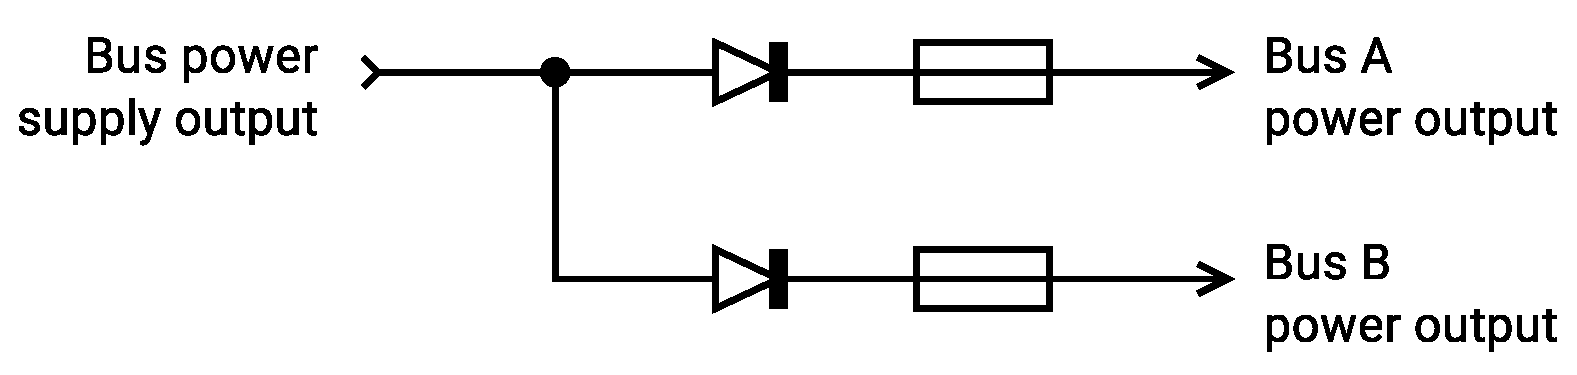
\includegraphics[width=0.6\textwidth]{physical_layer/redundant_bus_power_source}
	\caption{Simplified conceptual power sourcing node design schematic.\label{fig:phy_redundant_bus_power_source}}
\end{figure}

\chapter{List of standard data types}

This chapter contains the full list of standard data types defined by the UAVCAN specification.
The source text of the DSDL data type definitions provided here is also available via the
official project website at \href{http://uavcan.org}{uavcan.org}.

Regulated non-standard definitions\footnote{I.e., public definitions contributed by vendors and other users
of the specification, as explained in section \ref{sec:basic_concepts_data_type_regulation}.}
are intentionally not included in this list, as they are of limited importance for the specification.

Each definition is provided with a length information table for convenience,
where the minimum and maximum serialized length is shown in several units:
bits, bytes (octets), and transport frames for some of the supported transport protocols.
The acronym \emph{MTU} used in the length information tables stands for
\emph{maximum transmission unit}, which is the maximum amount of data, in bytes (octets, eight bits per byte),
that fits into one transport frame for the specific transport protocol.

The index table \ref{table:dsdl:uavcan} is provided before the definitions for ease of navigation.

\clearpage\DSDL{uavcan.*}


\end{document}
